% Seminar 3: α-stable distributions
% Statistics of Financial Markets -- Bachelor's programme, Bucharest University of Economic Studies
% GENERATED by latex/build_seminar3.py -- edit the generator, not this file.
% Student version by default; the instructor version is the *_solutions.tex wrapper.
\makeatletter\@ifundefined{ifsolutions}{\expandafter\newif\csname ifsolutions\endcsname}{}\makeatother

\newcommand{\coursename}{Statistics of Financial Markets}
% Preambul comun SFM -- Statistica piețelor financiare / Statistics of Financial Markets (Beamer, 16:9)
% Același design ca MFM. Înainte de % Preambul comun SFM -- Statistica piețelor financiare / Statistics of Financial Markets (Beamer, 16:9)
% Același design ca MFM. Înainte de % Preambul comun SFM -- Statistica piețelor financiare / Statistics of Financial Markets (Beamer, 16:9)
% Același design ca MFM. Înainte de \input{../../latex/preamble} se definește
%   \newcommand{\coursename}{Statistics of Financial Markets}      (EN)
%   \newcommand{\coursename}{Statistica piețelor financiare}       (RO)  și  \def\sfmlang{ro}
% Fișierele .tex se află în EN/Courses, EN/Seminars, RO/Cursuri, RO/Seminarii (două niveluri sub rădăcină).
% Deck-urile sînt generate de latex/build_chapterN.py / build_seminarN.py (vezi latex/sfm_build.py).

\documentclass[9pt, aspectratio=169, t]{beamer}
\providecommand{\coursename}{Statistics of Financial Markets}

% Ensure content fits on slides
\setbeamersize{text margin left=8mm, text margin right=8mm}

%=============================================================================
% THEME AND STYLE CONFIGURATION
%=============================================================================
\usetheme{default}
% Using default theme for clean header/footer control

% Color Palette (matching Redispatch PDF)
\definecolor{MainBlue}{RGB}{26, 58, 110}
\definecolor{AccentBlue}{RGB}{26, 58, 110}
\definecolor{IDAred}{RGB}{205, 0, 0}
\definecolor{DarkGray}{RGB}{51, 51, 51}
\definecolor{MediumGray}{RGB}{128, 128, 128}
\definecolor{LightGray}{RGB}{248, 248, 248}
\definecolor{VeryLightGray}{RGB}{235, 235, 235}
\definecolor{KeynoteGray}{RGB}{218, 218, 218}
\definecolor{SectionGray}{RGB}{120, 120, 120}
\definecolor{FooterGray}{RGB}{100, 100, 100}
\definecolor{Crimson}{RGB}{220, 53, 69}
\definecolor{Forest}{RGB}{46, 125, 50}
\definecolor{Amber}{RGB}{181, 133, 63}
\definecolor{Orange}{RGB}{230, 126, 34}
\definecolor{Purple}{RGB}{142, 68, 173}

% Gradient background (exact Keynote 315° gradient: white to RGB 218,218,218)
\setbeamertemplate{background}{%
    \begin{tikzpicture}[remember picture, overlay]
        \shade[shading=axis, shading angle=315,
        top color=white, bottom color=KeynoteGray]
        (current page.south west) rectangle (current page.north east);
    \end{tikzpicture}%
}
% Fallback solid color for compatibility
\setbeamercolor{background canvas}{bg=}

\setbeamercolor{palette primary}{bg=MainBlue, fg=white}
\setbeamercolor{palette secondary}{bg=MainBlue!85, fg=white}
\setbeamercolor{palette tertiary}{bg=MainBlue!70, fg=white}
\setbeamercolor{structure}{fg=MainBlue}
\setbeamercolor{title}{fg=IDAred}
\setbeamercolor{frametitle}{fg=IDAred, bg=}
\setbeamercolor{block title}{bg=MainBlue, fg=white}
\setbeamercolor{block body}{bg=VeryLightGray, fg=DarkGray}
\setbeamercolor{block title alerted}{bg=Crimson, fg=white}
\setbeamercolor{block body alerted}{bg=Crimson!8, fg=DarkGray}
\setbeamercolor{block title example}{bg=Forest, fg=white}
\setbeamercolor{block body example}{bg=Forest!8, fg=DarkGray}
\setbeamercolor{item}{fg=MainBlue}

% Footer colors (override Madrid theme blue)
\setbeamercolor{author in head/foot}{fg=FooterGray, bg=}
\setbeamercolor{title in head/foot}{fg=FooterGray, bg=}
\setbeamercolor{date in head/foot}{fg=FooterGray, bg=}
\setbeamercolor{section in head/foot}{fg=FooterGray, bg=}
\setbeamercolor{subsection in head/foot}{fg=FooterGray, bg=}

% Bullet styles (apply everywhere including blocks)
\setbeamertemplate{itemize item}{\color{MainBlue}$\boxdot$}
\setbeamertemplate{itemize subitem}{\color{MainBlue}$\blacktriangleright$}
\setbeamertemplate{itemize subsubitem}{\color{MainBlue}\tiny$\bullet$}
\setbeamertemplate{itemize/enumerate body begin}{\normalsize}
\setbeamertemplate{itemize/enumerate subbody begin}{\normalsize}

% Item spacing - compact style
\setlength{\leftmargini}{10pt}       % Level 1: minimal indent
\setlength{\leftmarginii}{10pt}      % Level 2: minimal additional indent
% Compact list spacing (zero extra space before/after lists in blocks)
\makeatletter
\def\@listi{\leftmargin\leftmargini \topsep 0pt \parsep 0pt \itemsep 0pt}
\def\@listii{\leftmargin\leftmarginii \topsep 0pt \parsep 0pt \itemsep 0pt}
\makeatother

\setbeamertemplate{navigation symbols}{}

%=============================================================================
% CUSTOM HEADLINE
%=============================================================================
\setbeamertemplate{headline}{%
    \vskip10pt%
    \hbox to \paperwidth{%
        \hskip0.5cm%
        {\small\color{FooterGray}\renewcommand{\hyperlink}[2]{##2}\insertsectionhead}%
        \hfill%
        \textcolor{FooterGray}{\small\insertframenumber}%
        \hskip0.5cm%
    }%
    \vskip4pt%
    {\color{FooterGray}\hrule height 0.4pt}%
}

%=============================================================================
% CUSTOM FOOTER
%=============================================================================
\usepackage{fontawesome5}

\setbeamertemplate{footline}{%
    {\color{FooterGray}\hrule height 0.4pt}%
    \vskip4pt%
    \hbox to \paperwidth{%
        \hskip0.5cm%
        \textcolor{FooterGray}{\small\coursename}%
        \hfill%
        \raisebox{-0.1em}{%
            \begin{tikzpicture}[x=0.08em, y=0.08em, line width=0.4pt]
                \draw[FooterGray] (0,3) -- (1,4) -- (2,3.5) -- (3,5) -- (4,4) -- (5,6) -- (6,5.5) -- (7,4) -- (8,5) -- (9,7) -- (10,6) -- (11,5) -- (12,6.5) -- (13,8) -- (14,7) -- (15,6) -- (16,7.5) -- (17,9) -- (18,8) -- (19,7) -- (20,8.5) -- (21,10) -- (22,9) -- (23,8) -- (24,9.5);
            \end{tikzpicture}%
        }%
        \hskip0.5cm%
    }%
    \vskip6pt%
}

%=============================================================================
% PACKAGES
%=============================================================================
\usepackage[utf8]{inputenc}
\DeclareUnicodeCharacter{03B1}{\ensuremath{\alpha}}
\usepackage[T1]{fontenc}
\usepackage{amsmath, amssymb, amsthm}
\usepackage{mathtools}
\usepackage{bm}
\usepackage{tikz}
\usetikzlibrary{arrows.meta, positioning, shapes, calc, decorations.pathreplacing, shadings}
\usepackage{booktabs}
\usepackage{multirow}
\usepackage{array}
\usepackage{graphicx}
\usepackage{hyperref}
\usepackage{colortbl}
\usepackage{listings}
\lstset{language=Python, basicstyle=\ttfamily\scriptsize, keywordstyle=\color{MainBlue}\bfseries,
  commentstyle=\color{Forest}, stringstyle=\color{Crimson}, breaklines=true,
  frame=none, backgroundcolor=\color{VeryLightGray}, xleftmargin=2mm}
\hypersetup{colorlinks=true, linkcolor=MainBlue, urlcolor=MainBlue}
\graphicspath{{../../logos/}{../../charts/}{../../photos/}}
\usepackage{xcolor}
\hfuzz=2pt  % Suppress tiny overfull warnings (<2pt)
\vfuzz=2pt  % Suppress tiny vertical overfull warnings (<2pt)

%=============================================================================
% QUANTLET COMMANDS
%   \quantlet{<displayed name>}{<url>}       (generic, compatible with the older SFM decks)
%   \sfmquantlet{Ch_05}{SFM_ch5_garch}       -> https://github.com/danpele/SFM/tree/main/Quantlets/Ch_05/SFM_ch5_garch
%   \qlurl{<folder>} is defined per chapter by the generator (Quantlets/Ch_NN/<folder>)
%=============================================================================
\newcommand{\sfmrepo}{https://github.com/danpele/SFM}
\newcommand{\sfmqlbase}{https://github.com/danpele/SFM/tree/main/Quantlets}
\newcommand{\quantlet}[2]{%
    \hfill\href{#2}{%
        \raisebox{-0.15em}{
\includegraphics[height=0.7em]{ql_logo.png}}%
        \textcolor{MainBlue}{\tiny\ #1}%
    }%
}
\newcommand{\sfmquantlet}[2]{\quantlet{\detokenize{#2}}{\sfmqlbase/#1/#2}}

%=============================================================================
% NOTEBOOKS (Google Colab)
%   \colaburl{notebooks/EN/chapter5_seminar_notebook.ipynb} -> the Colab link of a file in the SFM repo
%   \nb: the chapter notebook (each seminar deck redefines it with \renewcommand)
%=============================================================================
\newcommand{\colaburl}[1]{https://colab.research.google.com/github/danpele/SFM/blob/main/#1}
\newcommand{\nb}{https://colab.research.google.com/github/danpele/SFM/tree/main/notebooks/EN}
\newcommand{\nbname}{notebooks/EN}

%=============================================================================
% SLIDE HELPERS (used by the generators; the same as in MFM)
%=============================================================================
% local font size for list bodies (the preamble forces \normalsize)
\newcommand{\itemsize}[1]{\setbeamertemplate{itemize/enumerate body begin}{#1}\setbeamertemplate{itemize/enumerate subbody begin}{#1}}
\newcommand{\intitle}[1]{{\hypersetup{urlcolor=white}#1}}   % white links inside coloured title bars
\newcommand{\imgcap}[1]{{\scriptsize #1}\\[0.5mm]}          % caption under a photo
\newcommand{\imgcredit}[2]{{\tiny\color{FooterGray}\href{#1}{#2}}}   % image credit: source URL, author/licence
\newcommand{\aiprompt}[1]{{\ttfamily\color{MainBlue}#1}}     % a prompt to an AI assistant

%=============================================================================
% SEMINARS: student version by default; the instructor wrapper *_solutions.tex sets \solutionstrue
%=============================================================================
\makeatletter\@ifundefined{ifsolutions}{\expandafter\newif\csname ifsolutions\endcsname}{}\makeatother
\newcommand{\solonly}[1]{\ifsolutions #1\fi}
\newcommand{\propsub}{\ifsolutions\else\framesubtitle{\ifdefined\sfmlang Rezolvarea se discută la seminar\else Solution discussed in class\fi}\fi}

%=============================================================================
% APPENDIX AND CHAPTER LINKS (latex/appendix_links.py writes the calls; it also re-declares these
% macros before \begin{document}, so the decks compile with or without this preamble block)
%=============================================================================
\providecommand{\sfmapplink}[3]{\hypertarget{#2}{}\hyperlink{#1}{\beamergotobutton{#3}}}
\providecommand{\sfmappback}[2]{\begin{tikzpicture}[remember picture,overlay]\node[anchor=south east] at ([xshift=-3mm,yshift=7mm]current page.south east){\hyperlink{#1}{\beamerreturnbutton{#2}}};\end{tikzpicture}}
\providecommand{\sfmchlink}[2]{\href{#1}{#2}}
\providecommand{\sfmchlinkt}[2]{\href{#1}{\usebeamercolor[fg]{frametitle}#2}}

%=============================================================================
% QUANTINAR COMMAND: link către un curs Quantinar (subiecte avansate)
%=============================================================================
\newcommand{\quantinar}[2]{%
    \href{#2}{%
        \raisebox{-0.15em}{
\includegraphics[height=0.8em]{qr_logo.png}}%
        \textcolor{MainBlue}{\scriptsize\ #1}%
    }%
}

%=============================================================================
% CUSTOM TITLE PAGE
%=============================================================================
\defbeamertemplate*{title page}{hybrid}[1][]
{
    \vspace{0.2cm}
    % Logos row - top header (with clickable links)
    \begin{center}
        \href{https://www.ase.ro}{
\includegraphics[height=1.0cm]{ase_logo.png}}\hspace{0.3cm}%
        \href{https://theida.net}{
\includegraphics[height=1.0cm]{ida_logo.png}}\hspace{0.3cm}%
        \href{https://blockchain-research-center.com}{
\includegraphics[height=1.0cm]{brc_logo.png}}\hspace{0.3cm}%
        \href{https://www.ai4efin.ase.ro}{
\includegraphics[height=1.0cm]{ai4efin_logo.png}}\hspace{0.3cm}%
        \href{https://ipe.ro/new}{
\includegraphics[height=1.0cm]{acad_logo.png}}\hspace{0.3cm}%
        \href{https://www.digital-finance-msca.com}{
\includegraphics[height=1.0cm]{msca_logo.png}}%
    \end{center}

    \vspace{0.6cm}

    % Main title with Q logos on sides (with clickable links)
    \begin{center}
        \begin{minipage}{0.1\textwidth}
            \centering
            \href{https://quantlet.com}{
\includegraphics[height=1.1cm]{ql_logo.png}}
        \end{minipage}%
        \begin{minipage}{0.78\textwidth}
            \centering
            {\LARGE\bfseries\usebeamercolor[fg]{title}\inserttitle}

            \vspace{0.3cm}

            {\usebeamerfont{subtitle}\usebeamercolor[fg]{title}\insertsubtitle}
        \end{minipage}%
        \begin{minipage}{0.1\textwidth}
            \centering
            \href{https://quantinar.com}{
\includegraphics[height=1.1cm]{qr_logo.png}}
        \end{minipage}
    \end{center}

    \vspace{0.6cm}

    % Authors (left aligned)
    \hspace{0.5cm}{\usebeamerfont{author}\insertauthor}

    \vspace{0.3cm}

    % Institute/Affiliations (left aligned)
    \hspace{0.5cm}\begin{minipage}[t]{0.9\textwidth}
        \raggedright\small\insertinstitute
    \end{minipage}
}

%=============================================================================
% THEOREM ENVIRONMENTS
%=============================================================================
\theoremstyle{definition}
\setbeamertemplate{theorems}[numbered]
\ifdefined\sfmlang
\newtheorem{defn}{Definiție}
\newtheorem{thm}{Teoremă}
\newtheorem{prop}{Propoziție}
\newtheorem{rmk}{Observație}
\else
\newtheorem{defn}{Definition}
\newtheorem{thm}{Theorem}
\newtheorem{prop}{Proposition}
\newtheorem{rmk}{Remark}
\fi

%=============================================================================
% CENTRED MINIPAGE (no extra vertical space)
%=============================================================================
\newenvironment{cminipage}[1]{%
    \par\noindent\hfill\begin{minipage}{#1}\ignorespaces
}{%
    \end{minipage}\hfill\null\par
}

%=============================================================================
% CUSTOM COMMANDS
%=============================================================================
\newcommand{\E}{\mathbb{E}}
\newcommand{\Var}{\text{Var}}
\newcommand{\Cov}{\text{Cov}}
\newcommand{\Corr}{\text{Corr}}
\newcommand{\R}{\mathbb{R}}
\newcommand{\N}{\mathbb{N}}
\newcommand{\Z}{\mathbb{Z}}
\newcommand{\B}{\mathbf{B}}
\newcommand{\imark}{\textcolor{MainBlue}{\textbullet}}
\newcommand{\RMSE}{\text{RMSE}}
\newcommand{\MAE}{\text{MAE}}
\newcommand{\MAPE}{\text{MAPE}}

 se definește
%   \newcommand{\coursename}{Statistics of Financial Markets}      (EN)
%   \newcommand{\coursename}{Statistica piețelor financiare}       (RO)  și  \def\sfmlang{ro}
% Fișierele .tex se află în EN/Courses, EN/Seminars, RO/Cursuri, RO/Seminarii (două niveluri sub rădăcină).
% Deck-urile sînt generate de latex/build_chapterN.py / build_seminarN.py (vezi latex/sfm_build.py).

\documentclass[9pt, aspectratio=169, t]{beamer}
\providecommand{\coursename}{Statistics of Financial Markets}

% Ensure content fits on slides
\setbeamersize{text margin left=8mm, text margin right=8mm}

%=============================================================================
% THEME AND STYLE CONFIGURATION
%=============================================================================
\usetheme{default}
% Using default theme for clean header/footer control

% Color Palette (matching Redispatch PDF)
\definecolor{MainBlue}{RGB}{26, 58, 110}
\definecolor{AccentBlue}{RGB}{26, 58, 110}
\definecolor{IDAred}{RGB}{205, 0, 0}
\definecolor{DarkGray}{RGB}{51, 51, 51}
\definecolor{MediumGray}{RGB}{128, 128, 128}
\definecolor{LightGray}{RGB}{248, 248, 248}
\definecolor{VeryLightGray}{RGB}{235, 235, 235}
\definecolor{KeynoteGray}{RGB}{218, 218, 218}
\definecolor{SectionGray}{RGB}{120, 120, 120}
\definecolor{FooterGray}{RGB}{100, 100, 100}
\definecolor{Crimson}{RGB}{220, 53, 69}
\definecolor{Forest}{RGB}{46, 125, 50}
\definecolor{Amber}{RGB}{181, 133, 63}
\definecolor{Orange}{RGB}{230, 126, 34}
\definecolor{Purple}{RGB}{142, 68, 173}

% Gradient background (exact Keynote 315° gradient: white to RGB 218,218,218)
\setbeamertemplate{background}{%
    \begin{tikzpicture}[remember picture, overlay]
        \shade[shading=axis, shading angle=315,
        top color=white, bottom color=KeynoteGray]
        (current page.south west) rectangle (current page.north east);
    \end{tikzpicture}%
}
% Fallback solid color for compatibility
\setbeamercolor{background canvas}{bg=}

\setbeamercolor{palette primary}{bg=MainBlue, fg=white}
\setbeamercolor{palette secondary}{bg=MainBlue!85, fg=white}
\setbeamercolor{palette tertiary}{bg=MainBlue!70, fg=white}
\setbeamercolor{structure}{fg=MainBlue}
\setbeamercolor{title}{fg=IDAred}
\setbeamercolor{frametitle}{fg=IDAred, bg=}
\setbeamercolor{block title}{bg=MainBlue, fg=white}
\setbeamercolor{block body}{bg=VeryLightGray, fg=DarkGray}
\setbeamercolor{block title alerted}{bg=Crimson, fg=white}
\setbeamercolor{block body alerted}{bg=Crimson!8, fg=DarkGray}
\setbeamercolor{block title example}{bg=Forest, fg=white}
\setbeamercolor{block body example}{bg=Forest!8, fg=DarkGray}
\setbeamercolor{item}{fg=MainBlue}

% Footer colors (override Madrid theme blue)
\setbeamercolor{author in head/foot}{fg=FooterGray, bg=}
\setbeamercolor{title in head/foot}{fg=FooterGray, bg=}
\setbeamercolor{date in head/foot}{fg=FooterGray, bg=}
\setbeamercolor{section in head/foot}{fg=FooterGray, bg=}
\setbeamercolor{subsection in head/foot}{fg=FooterGray, bg=}

% Bullet styles (apply everywhere including blocks)
\setbeamertemplate{itemize item}{\color{MainBlue}$\boxdot$}
\setbeamertemplate{itemize subitem}{\color{MainBlue}$\blacktriangleright$}
\setbeamertemplate{itemize subsubitem}{\color{MainBlue}\tiny$\bullet$}
\setbeamertemplate{itemize/enumerate body begin}{\normalsize}
\setbeamertemplate{itemize/enumerate subbody begin}{\normalsize}

% Item spacing - compact style
\setlength{\leftmargini}{10pt}       % Level 1: minimal indent
\setlength{\leftmarginii}{10pt}      % Level 2: minimal additional indent
% Compact list spacing (zero extra space before/after lists in blocks)
\makeatletter
\def\@listi{\leftmargin\leftmargini \topsep 0pt \parsep 0pt \itemsep 0pt}
\def\@listii{\leftmargin\leftmarginii \topsep 0pt \parsep 0pt \itemsep 0pt}
\makeatother

\setbeamertemplate{navigation symbols}{}

%=============================================================================
% CUSTOM HEADLINE
%=============================================================================
\setbeamertemplate{headline}{%
    \vskip10pt%
    \hbox to \paperwidth{%
        \hskip0.5cm%
        {\small\color{FooterGray}\renewcommand{\hyperlink}[2]{##2}\insertsectionhead}%
        \hfill%
        \textcolor{FooterGray}{\small\insertframenumber}%
        \hskip0.5cm%
    }%
    \vskip4pt%
    {\color{FooterGray}\hrule height 0.4pt}%
}

%=============================================================================
% CUSTOM FOOTER
%=============================================================================
\usepackage{fontawesome5}

\setbeamertemplate{footline}{%
    {\color{FooterGray}\hrule height 0.4pt}%
    \vskip4pt%
    \hbox to \paperwidth{%
        \hskip0.5cm%
        \textcolor{FooterGray}{\small\coursename}%
        \hfill%
        \raisebox{-0.1em}{%
            \begin{tikzpicture}[x=0.08em, y=0.08em, line width=0.4pt]
                \draw[FooterGray] (0,3) -- (1,4) -- (2,3.5) -- (3,5) -- (4,4) -- (5,6) -- (6,5.5) -- (7,4) -- (8,5) -- (9,7) -- (10,6) -- (11,5) -- (12,6.5) -- (13,8) -- (14,7) -- (15,6) -- (16,7.5) -- (17,9) -- (18,8) -- (19,7) -- (20,8.5) -- (21,10) -- (22,9) -- (23,8) -- (24,9.5);
            \end{tikzpicture}%
        }%
        \hskip0.5cm%
    }%
    \vskip6pt%
}

%=============================================================================
% PACKAGES
%=============================================================================
\usepackage[utf8]{inputenc}
\DeclareUnicodeCharacter{03B1}{\ensuremath{\alpha}}
\usepackage[T1]{fontenc}
\usepackage{amsmath, amssymb, amsthm}
\usepackage{mathtools}
\usepackage{bm}
\usepackage{tikz}
\usetikzlibrary{arrows.meta, positioning, shapes, calc, decorations.pathreplacing, shadings}
\usepackage{booktabs}
\usepackage{multirow}
\usepackage{array}
\usepackage{graphicx}
\usepackage{hyperref}
\usepackage{colortbl}
\usepackage{listings}
\lstset{language=Python, basicstyle=\ttfamily\scriptsize, keywordstyle=\color{MainBlue}\bfseries,
  commentstyle=\color{Forest}, stringstyle=\color{Crimson}, breaklines=true,
  frame=none, backgroundcolor=\color{VeryLightGray}, xleftmargin=2mm}
\hypersetup{colorlinks=true, linkcolor=MainBlue, urlcolor=MainBlue}
\graphicspath{{../../logos/}{../../charts/}{../../photos/}}
\usepackage{xcolor}
\hfuzz=2pt  % Suppress tiny overfull warnings (<2pt)
\vfuzz=2pt  % Suppress tiny vertical overfull warnings (<2pt)

%=============================================================================
% QUANTLET COMMANDS
%   \quantlet{<displayed name>}{<url>}       (generic, compatible with the older SFM decks)
%   \sfmquantlet{Ch_05}{SFM_ch5_garch}       -> https://github.com/danpele/SFM/tree/main/Quantlets/Ch_05/SFM_ch5_garch
%   \qlurl{<folder>} is defined per chapter by the generator (Quantlets/Ch_NN/<folder>)
%=============================================================================
\newcommand{\sfmrepo}{https://github.com/danpele/SFM}
\newcommand{\sfmqlbase}{https://github.com/danpele/SFM/tree/main/Quantlets}
\newcommand{\quantlet}[2]{%
    \hfill\href{#2}{%
        \raisebox{-0.15em}{
\includegraphics[height=0.7em]{ql_logo.png}}%
        \textcolor{MainBlue}{\tiny\ #1}%
    }%
}
\newcommand{\sfmquantlet}[2]{\quantlet{\detokenize{#2}}{\sfmqlbase/#1/#2}}

%=============================================================================
% NOTEBOOKS (Google Colab)
%   \colaburl{notebooks/EN/chapter5_seminar_notebook.ipynb} -> the Colab link of a file in the SFM repo
%   \nb: the chapter notebook (each seminar deck redefines it with \renewcommand)
%=============================================================================
\newcommand{\colaburl}[1]{https://colab.research.google.com/github/danpele/SFM/blob/main/#1}
\newcommand{\nb}{https://colab.research.google.com/github/danpele/SFM/tree/main/notebooks/EN}
\newcommand{\nbname}{notebooks/EN}

%=============================================================================
% SLIDE HELPERS (used by the generators; the same as in MFM)
%=============================================================================
% local font size for list bodies (the preamble forces \normalsize)
\newcommand{\itemsize}[1]{\setbeamertemplate{itemize/enumerate body begin}{#1}\setbeamertemplate{itemize/enumerate subbody begin}{#1}}
\newcommand{\intitle}[1]{{\hypersetup{urlcolor=white}#1}}   % white links inside coloured title bars
\newcommand{\imgcap}[1]{{\scriptsize #1}\\[0.5mm]}          % caption under a photo
\newcommand{\imgcredit}[2]{{\tiny\color{FooterGray}\href{#1}{#2}}}   % image credit: source URL, author/licence
\newcommand{\aiprompt}[1]{{\ttfamily\color{MainBlue}#1}}     % a prompt to an AI assistant

%=============================================================================
% SEMINARS: student version by default; the instructor wrapper *_solutions.tex sets \solutionstrue
%=============================================================================
\makeatletter\@ifundefined{ifsolutions}{\expandafter\newif\csname ifsolutions\endcsname}{}\makeatother
\newcommand{\solonly}[1]{\ifsolutions #1\fi}
\newcommand{\propsub}{\ifsolutions\else\framesubtitle{\ifdefined\sfmlang Rezolvarea se discută la seminar\else Solution discussed in class\fi}\fi}

%=============================================================================
% APPENDIX AND CHAPTER LINKS (latex/appendix_links.py writes the calls; it also re-declares these
% macros before \begin{document}, so the decks compile with or without this preamble block)
%=============================================================================
\providecommand{\sfmapplink}[3]{\hypertarget{#2}{}\hyperlink{#1}{\beamergotobutton{#3}}}
\providecommand{\sfmappback}[2]{\begin{tikzpicture}[remember picture,overlay]\node[anchor=south east] at ([xshift=-3mm,yshift=7mm]current page.south east){\hyperlink{#1}{\beamerreturnbutton{#2}}};\end{tikzpicture}}
\providecommand{\sfmchlink}[2]{\href{#1}{#2}}
\providecommand{\sfmchlinkt}[2]{\href{#1}{\usebeamercolor[fg]{frametitle}#2}}

%=============================================================================
% QUANTINAR COMMAND: link către un curs Quantinar (subiecte avansate)
%=============================================================================
\newcommand{\quantinar}[2]{%
    \href{#2}{%
        \raisebox{-0.15em}{
\includegraphics[height=0.8em]{qr_logo.png}}%
        \textcolor{MainBlue}{\scriptsize\ #1}%
    }%
}

%=============================================================================
% CUSTOM TITLE PAGE
%=============================================================================
\defbeamertemplate*{title page}{hybrid}[1][]
{
    \vspace{0.2cm}
    % Logos row - top header (with clickable links)
    \begin{center}
        \href{https://www.ase.ro}{
\includegraphics[height=1.0cm]{ase_logo.png}}\hspace{0.3cm}%
        \href{https://theida.net}{
\includegraphics[height=1.0cm]{ida_logo.png}}\hspace{0.3cm}%
        \href{https://blockchain-research-center.com}{
\includegraphics[height=1.0cm]{brc_logo.png}}\hspace{0.3cm}%
        \href{https://www.ai4efin.ase.ro}{
\includegraphics[height=1.0cm]{ai4efin_logo.png}}\hspace{0.3cm}%
        \href{https://ipe.ro/new}{
\includegraphics[height=1.0cm]{acad_logo.png}}\hspace{0.3cm}%
        \href{https://www.digital-finance-msca.com}{
\includegraphics[height=1.0cm]{msca_logo.png}}%
    \end{center}

    \vspace{0.6cm}

    % Main title with Q logos on sides (with clickable links)
    \begin{center}
        \begin{minipage}{0.1\textwidth}
            \centering
            \href{https://quantlet.com}{
\includegraphics[height=1.1cm]{ql_logo.png}}
        \end{minipage}%
        \begin{minipage}{0.78\textwidth}
            \centering
            {\LARGE\bfseries\usebeamercolor[fg]{title}\inserttitle}

            \vspace{0.3cm}

            {\usebeamerfont{subtitle}\usebeamercolor[fg]{title}\insertsubtitle}
        \end{minipage}%
        \begin{minipage}{0.1\textwidth}
            \centering
            \href{https://quantinar.com}{
\includegraphics[height=1.1cm]{qr_logo.png}}
        \end{minipage}
    \end{center}

    \vspace{0.6cm}

    % Authors (left aligned)
    \hspace{0.5cm}{\usebeamerfont{author}\insertauthor}

    \vspace{0.3cm}

    % Institute/Affiliations (left aligned)
    \hspace{0.5cm}\begin{minipage}[t]{0.9\textwidth}
        \raggedright\small\insertinstitute
    \end{minipage}
}

%=============================================================================
% THEOREM ENVIRONMENTS
%=============================================================================
\theoremstyle{definition}
\setbeamertemplate{theorems}[numbered]
\ifdefined\sfmlang
\newtheorem{defn}{Definiție}
\newtheorem{thm}{Teoremă}
\newtheorem{prop}{Propoziție}
\newtheorem{rmk}{Observație}
\else
\newtheorem{defn}{Definition}
\newtheorem{thm}{Theorem}
\newtheorem{prop}{Proposition}
\newtheorem{rmk}{Remark}
\fi

%=============================================================================
% CENTRED MINIPAGE (no extra vertical space)
%=============================================================================
\newenvironment{cminipage}[1]{%
    \par\noindent\hfill\begin{minipage}{#1}\ignorespaces
}{%
    \end{minipage}\hfill\null\par
}

%=============================================================================
% CUSTOM COMMANDS
%=============================================================================
\newcommand{\E}{\mathbb{E}}
\newcommand{\Var}{\text{Var}}
\newcommand{\Cov}{\text{Cov}}
\newcommand{\Corr}{\text{Corr}}
\newcommand{\R}{\mathbb{R}}
\newcommand{\N}{\mathbb{N}}
\newcommand{\Z}{\mathbb{Z}}
\newcommand{\B}{\mathbf{B}}
\newcommand{\imark}{\textcolor{MainBlue}{\textbullet}}
\newcommand{\RMSE}{\text{RMSE}}
\newcommand{\MAE}{\text{MAE}}
\newcommand{\MAPE}{\text{MAPE}}

 se definește
%   \newcommand{\coursename}{Statistics of Financial Markets}      (EN)
%   \newcommand{\coursename}{Statistica piețelor financiare}       (RO)  și  \def\sfmlang{ro}
% Fișierele .tex se află în EN/Courses, EN/Seminars, RO/Cursuri, RO/Seminarii (două niveluri sub rădăcină).
% Deck-urile sînt generate de latex/build_chapterN.py / build_seminarN.py (vezi latex/sfm_build.py).

\documentclass[9pt, aspectratio=169, t]{beamer}
\providecommand{\coursename}{Statistics of Financial Markets}

% Ensure content fits on slides
\setbeamersize{text margin left=8mm, text margin right=8mm}

%=============================================================================
% THEME AND STYLE CONFIGURATION
%=============================================================================
\usetheme{default}
% Using default theme for clean header/footer control

% Color Palette (matching Redispatch PDF)
\definecolor{MainBlue}{RGB}{26, 58, 110}
\definecolor{AccentBlue}{RGB}{26, 58, 110}
\definecolor{IDAred}{RGB}{205, 0, 0}
\definecolor{DarkGray}{RGB}{51, 51, 51}
\definecolor{MediumGray}{RGB}{128, 128, 128}
\definecolor{LightGray}{RGB}{248, 248, 248}
\definecolor{VeryLightGray}{RGB}{235, 235, 235}
\definecolor{KeynoteGray}{RGB}{218, 218, 218}
\definecolor{SectionGray}{RGB}{120, 120, 120}
\definecolor{FooterGray}{RGB}{100, 100, 100}
\definecolor{Crimson}{RGB}{220, 53, 69}
\definecolor{Forest}{RGB}{46, 125, 50}
\definecolor{Amber}{RGB}{181, 133, 63}
\definecolor{Orange}{RGB}{230, 126, 34}
\definecolor{Purple}{RGB}{142, 68, 173}

% Gradient background (exact Keynote 315° gradient: white to RGB 218,218,218)
\setbeamertemplate{background}{%
    \begin{tikzpicture}[remember picture, overlay]
        \shade[shading=axis, shading angle=315,
        top color=white, bottom color=KeynoteGray]
        (current page.south west) rectangle (current page.north east);
    \end{tikzpicture}%
}
% Fallback solid color for compatibility
\setbeamercolor{background canvas}{bg=}

\setbeamercolor{palette primary}{bg=MainBlue, fg=white}
\setbeamercolor{palette secondary}{bg=MainBlue!85, fg=white}
\setbeamercolor{palette tertiary}{bg=MainBlue!70, fg=white}
\setbeamercolor{structure}{fg=MainBlue}
\setbeamercolor{title}{fg=IDAred}
\setbeamercolor{frametitle}{fg=IDAred, bg=}
\setbeamercolor{block title}{bg=MainBlue, fg=white}
\setbeamercolor{block body}{bg=VeryLightGray, fg=DarkGray}
\setbeamercolor{block title alerted}{bg=Crimson, fg=white}
\setbeamercolor{block body alerted}{bg=Crimson!8, fg=DarkGray}
\setbeamercolor{block title example}{bg=Forest, fg=white}
\setbeamercolor{block body example}{bg=Forest!8, fg=DarkGray}
\setbeamercolor{item}{fg=MainBlue}

% Footer colors (override Madrid theme blue)
\setbeamercolor{author in head/foot}{fg=FooterGray, bg=}
\setbeamercolor{title in head/foot}{fg=FooterGray, bg=}
\setbeamercolor{date in head/foot}{fg=FooterGray, bg=}
\setbeamercolor{section in head/foot}{fg=FooterGray, bg=}
\setbeamercolor{subsection in head/foot}{fg=FooterGray, bg=}

% Bullet styles (apply everywhere including blocks)
\setbeamertemplate{itemize item}{\color{MainBlue}$\boxdot$}
\setbeamertemplate{itemize subitem}{\color{MainBlue}$\blacktriangleright$}
\setbeamertemplate{itemize subsubitem}{\color{MainBlue}\tiny$\bullet$}
\setbeamertemplate{itemize/enumerate body begin}{\normalsize}
\setbeamertemplate{itemize/enumerate subbody begin}{\normalsize}

% Item spacing - compact style
\setlength{\leftmargini}{10pt}       % Level 1: minimal indent
\setlength{\leftmarginii}{10pt}      % Level 2: minimal additional indent
% Compact list spacing (zero extra space before/after lists in blocks)
\makeatletter
\def\@listi{\leftmargin\leftmargini \topsep 0pt \parsep 0pt \itemsep 0pt}
\def\@listii{\leftmargin\leftmarginii \topsep 0pt \parsep 0pt \itemsep 0pt}
\makeatother

\setbeamertemplate{navigation symbols}{}

%=============================================================================
% CUSTOM HEADLINE
%=============================================================================
\setbeamertemplate{headline}{%
    \vskip10pt%
    \hbox to \paperwidth{%
        \hskip0.5cm%
        {\small\color{FooterGray}\renewcommand{\hyperlink}[2]{##2}\insertsectionhead}%
        \hfill%
        \textcolor{FooterGray}{\small\insertframenumber}%
        \hskip0.5cm%
    }%
    \vskip4pt%
    {\color{FooterGray}\hrule height 0.4pt}%
}

%=============================================================================
% CUSTOM FOOTER
%=============================================================================
\usepackage{fontawesome5}

\setbeamertemplate{footline}{%
    {\color{FooterGray}\hrule height 0.4pt}%
    \vskip4pt%
    \hbox to \paperwidth{%
        \hskip0.5cm%
        \textcolor{FooterGray}{\small\coursename}%
        \hfill%
        \raisebox{-0.1em}{%
            \begin{tikzpicture}[x=0.08em, y=0.08em, line width=0.4pt]
                \draw[FooterGray] (0,3) -- (1,4) -- (2,3.5) -- (3,5) -- (4,4) -- (5,6) -- (6,5.5) -- (7,4) -- (8,5) -- (9,7) -- (10,6) -- (11,5) -- (12,6.5) -- (13,8) -- (14,7) -- (15,6) -- (16,7.5) -- (17,9) -- (18,8) -- (19,7) -- (20,8.5) -- (21,10) -- (22,9) -- (23,8) -- (24,9.5);
            \end{tikzpicture}%
        }%
        \hskip0.5cm%
    }%
    \vskip6pt%
}

%=============================================================================
% PACKAGES
%=============================================================================
\usepackage[utf8]{inputenc}
\DeclareUnicodeCharacter{03B1}{\ensuremath{\alpha}}
\usepackage[T1]{fontenc}
\usepackage{amsmath, amssymb, amsthm}
\usepackage{mathtools}
\usepackage{bm}
\usepackage{tikz}
\usetikzlibrary{arrows.meta, positioning, shapes, calc, decorations.pathreplacing, shadings}
\usepackage{booktabs}
\usepackage{multirow}
\usepackage{array}
\usepackage{graphicx}
\usepackage{hyperref}
\usepackage{colortbl}
\usepackage{listings}
\lstset{language=Python, basicstyle=\ttfamily\scriptsize, keywordstyle=\color{MainBlue}\bfseries,
  commentstyle=\color{Forest}, stringstyle=\color{Crimson}, breaklines=true,
  frame=none, backgroundcolor=\color{VeryLightGray}, xleftmargin=2mm}
\hypersetup{colorlinks=true, linkcolor=MainBlue, urlcolor=MainBlue}
\graphicspath{{../../logos/}{../../charts/}{../../photos/}}
\usepackage{xcolor}
\hfuzz=2pt  % Suppress tiny overfull warnings (<2pt)
\vfuzz=2pt  % Suppress tiny vertical overfull warnings (<2pt)

%=============================================================================
% QUANTLET COMMANDS
%   \quantlet{<displayed name>}{<url>}       (generic, compatible with the older SFM decks)
%   \sfmquantlet{Ch_05}{SFM_ch5_garch}       -> https://github.com/danpele/SFM/tree/main/Quantlets/Ch_05/SFM_ch5_garch
%   \qlurl{<folder>} is defined per chapter by the generator (Quantlets/Ch_NN/<folder>)
%=============================================================================
\newcommand{\sfmrepo}{https://github.com/danpele/SFM}
\newcommand{\sfmqlbase}{https://github.com/danpele/SFM/tree/main/Quantlets}
\newcommand{\quantlet}[2]{%
    \hfill\href{#2}{%
        \raisebox{-0.15em}{
\includegraphics[height=0.7em]{ql_logo.png}}%
        \textcolor{MainBlue}{\tiny\ #1}%
    }%
}
\newcommand{\sfmquantlet}[2]{\quantlet{\detokenize{#2}}{\sfmqlbase/#1/#2}}

%=============================================================================
% NOTEBOOKS (Google Colab)
%   \colaburl{notebooks/EN/chapter5_seminar_notebook.ipynb} -> the Colab link of a file in the SFM repo
%   \nb: the chapter notebook (each seminar deck redefines it with \renewcommand)
%=============================================================================
\newcommand{\colaburl}[1]{https://colab.research.google.com/github/danpele/SFM/blob/main/#1}
\newcommand{\nb}{https://colab.research.google.com/github/danpele/SFM/tree/main/notebooks/EN}
\newcommand{\nbname}{notebooks/EN}

%=============================================================================
% SLIDE HELPERS (used by the generators; the same as in MFM)
%=============================================================================
% local font size for list bodies (the preamble forces \normalsize)
\newcommand{\itemsize}[1]{\setbeamertemplate{itemize/enumerate body begin}{#1}\setbeamertemplate{itemize/enumerate subbody begin}{#1}}
\newcommand{\intitle}[1]{{\hypersetup{urlcolor=white}#1}}   % white links inside coloured title bars
\newcommand{\imgcap}[1]{{\scriptsize #1}\\[0.5mm]}          % caption under a photo
\newcommand{\imgcredit}[2]{{\tiny\color{FooterGray}\href{#1}{#2}}}   % image credit: source URL, author/licence
\newcommand{\aiprompt}[1]{{\ttfamily\color{MainBlue}#1}}     % a prompt to an AI assistant

%=============================================================================
% SEMINARS: student version by default; the instructor wrapper *_solutions.tex sets \solutionstrue
%=============================================================================
\makeatletter\@ifundefined{ifsolutions}{\expandafter\newif\csname ifsolutions\endcsname}{}\makeatother
\newcommand{\solonly}[1]{\ifsolutions #1\fi}
\newcommand{\propsub}{\ifsolutions\else\framesubtitle{\ifdefined\sfmlang Rezolvarea se discută la seminar\else Solution discussed in class\fi}\fi}

%=============================================================================
% APPENDIX AND CHAPTER LINKS (latex/appendix_links.py writes the calls; it also re-declares these
% macros before \begin{document}, so the decks compile with or without this preamble block)
%=============================================================================
\providecommand{\sfmapplink}[3]{\hypertarget{#2}{}\hyperlink{#1}{\beamergotobutton{#3}}}
\providecommand{\sfmappback}[2]{\begin{tikzpicture}[remember picture,overlay]\node[anchor=south east] at ([xshift=-3mm,yshift=7mm]current page.south east){\hyperlink{#1}{\beamerreturnbutton{#2}}};\end{tikzpicture}}
\providecommand{\sfmchlink}[2]{\href{#1}{#2}}
\providecommand{\sfmchlinkt}[2]{\href{#1}{\usebeamercolor[fg]{frametitle}#2}}

%=============================================================================
% QUANTINAR COMMAND: link către un curs Quantinar (subiecte avansate)
%=============================================================================
\newcommand{\quantinar}[2]{%
    \href{#2}{%
        \raisebox{-0.15em}{
\includegraphics[height=0.8em]{qr_logo.png}}%
        \textcolor{MainBlue}{\scriptsize\ #1}%
    }%
}

%=============================================================================
% CUSTOM TITLE PAGE
%=============================================================================
\defbeamertemplate*{title page}{hybrid}[1][]
{
    \vspace{0.2cm}
    % Logos row - top header (with clickable links)
    \begin{center}
        \href{https://www.ase.ro}{
\includegraphics[height=1.0cm]{ase_logo.png}}\hspace{0.3cm}%
        \href{https://theida.net}{
\includegraphics[height=1.0cm]{ida_logo.png}}\hspace{0.3cm}%
        \href{https://blockchain-research-center.com}{
\includegraphics[height=1.0cm]{brc_logo.png}}\hspace{0.3cm}%
        \href{https://www.ai4efin.ase.ro}{
\includegraphics[height=1.0cm]{ai4efin_logo.png}}\hspace{0.3cm}%
        \href{https://ipe.ro/new}{
\includegraphics[height=1.0cm]{acad_logo.png}}\hspace{0.3cm}%
        \href{https://www.digital-finance-msca.com}{
\includegraphics[height=1.0cm]{msca_logo.png}}%
    \end{center}

    \vspace{0.6cm}

    % Main title with Q logos on sides (with clickable links)
    \begin{center}
        \begin{minipage}{0.1\textwidth}
            \centering
            \href{https://quantlet.com}{
\includegraphics[height=1.1cm]{ql_logo.png}}
        \end{minipage}%
        \begin{minipage}{0.78\textwidth}
            \centering
            {\LARGE\bfseries\usebeamercolor[fg]{title}\inserttitle}

            \vspace{0.3cm}

            {\usebeamerfont{subtitle}\usebeamercolor[fg]{title}\insertsubtitle}
        \end{minipage}%
        \begin{minipage}{0.1\textwidth}
            \centering
            \href{https://quantinar.com}{
\includegraphics[height=1.1cm]{qr_logo.png}}
        \end{minipage}
    \end{center}

    \vspace{0.6cm}

    % Authors (left aligned)
    \hspace{0.5cm}{\usebeamerfont{author}\insertauthor}

    \vspace{0.3cm}

    % Institute/Affiliations (left aligned)
    \hspace{0.5cm}\begin{minipage}[t]{0.9\textwidth}
        \raggedright\small\insertinstitute
    \end{minipage}
}

%=============================================================================
% THEOREM ENVIRONMENTS
%=============================================================================
\theoremstyle{definition}
\setbeamertemplate{theorems}[numbered]
\ifdefined\sfmlang
\newtheorem{defn}{Definiție}
\newtheorem{thm}{Teoremă}
\newtheorem{prop}{Propoziție}
\newtheorem{rmk}{Observație}
\else
\newtheorem{defn}{Definition}
\newtheorem{thm}{Theorem}
\newtheorem{prop}{Proposition}
\newtheorem{rmk}{Remark}
\fi

%=============================================================================
% CENTRED MINIPAGE (no extra vertical space)
%=============================================================================
\newenvironment{cminipage}[1]{%
    \par\noindent\hfill\begin{minipage}{#1}\ignorespaces
}{%
    \end{minipage}\hfill\null\par
}

%=============================================================================
% CUSTOM COMMANDS
%=============================================================================
\newcommand{\E}{\mathbb{E}}
\newcommand{\Var}{\text{Var}}
\newcommand{\Cov}{\text{Cov}}
\newcommand{\Corr}{\text{Corr}}
\newcommand{\R}{\mathbb{R}}
\newcommand{\N}{\mathbb{N}}
\newcommand{\Z}{\mathbb{Z}}
\newcommand{\B}{\mathbf{B}}
\newcommand{\imark}{\textcolor{MainBlue}{\textbullet}}
\newcommand{\RMSE}{\text{RMSE}}
\newcommand{\MAE}{\text{MAE}}
\newcommand{\MAPE}{\text{MAPE}}



\newcommand{\qlurl}[1]{https://github.com/danpele/SFM/tree/main/Quantlets/Ch_03/#1}
\renewcommand{\nb}{\colaburl{notebooks/EN/chapter3_seminar_notebook.ipynb}}
\renewcommand{\nbname}{chapter3\_seminar\_notebook.ipynb}
% left column: full width in the student version, narrower next to the solution
\newcommand{\taskw}{\ifsolutions 0.47\textwidth\else 0.96\textwidth\fi}
\newcommand{\solw}{\ifsolutions 0.49\textwidth\else 0pt\fi}

\DeclareUnicodeCharacter{03B1}{\ensuremath{\alpha}}

% Clickable citations (DOIs verified via Crossref)

\newcommand{\refMandelbrot}{\href{https://doi.org/10.1086/294632}{Mandelbrot (1963)}}
\newcommand{\refFama}{\href{https://doi.org/10.1086/294743}{Fama (1965)}}
\newcommand{\refFamaRoll}{\href{https://doi.org/10.1080/01621459.1968.11009311}{Fama \& Roll (1968)}}
\newcommand{\refFamaRollB}{\href{https://doi.org/10.1080/01621459.1971.10482264}{Fama \& Roll (1971)}}
\newcommand{\refCMS}{\href{https://doi.org/10.1080/01621459.1976.10480344}{Chambers, Mallows \& Stuck (1976)}}
\newcommand{\refWeron}{\href{https://doi.org/10.1016/0167-7152(95)00113-1}{Weron (1996)}}
\newcommand{\refMcCulloch}{\href{https://doi.org/10.1080/03610918608812563}{McCulloch (1986)}}
\newcommand{\refNolanA}{\href{https://doi.org/10.1080/15326349708807450}{Nolan (1997)}}
\newcommand{\refNolan}{\href{https://doi.org/10.1007/978-3-030-52915-4}{Nolan (2020)}}
\newcommand{\refNolanML}{\href{https://doi.org/10.1007/978-1-4612-0197-7_17}{Nolan (2001)}}
\newcommand{\refST}{\href{https://doi.org/10.1201/9780203738818}{Samorodnitsky \& Taqqu (1994)}}
\newcommand{\refBHW}{\href{https://doi.org/10.1007/3-540-27395-6_1}{Borak, Härdle \& Weron (2005)}}
\newcommand{\refBMW}{\href{https://doi.org/10.1007/978-3-642-18062-0_1}{Borak, Misiorek \& Weron (2011)}}
\newcommand{\refFHH}{\href{https://doi.org/10.1007/978-3-030-13751-9}{Franke, Härdle \& Hafner (2019)}}
\newcommand{\refOfficer}{\href{https://doi.org/10.1080/01621459.1972.10481297}{Officer (1972)}}
\newcommand{\refBG}{\href{https://doi.org/10.1086/295634}{Blattberg \& Gonedes (1974)}}
\newcommand{\refAB}{\href{https://doi.org/10.1080/07350015.1988.10509636}{Akgiray \& Booth (1988)}}
\newcommand{\refLLW}{\href{https://doi.org/10.1080/07350015.1990.10509793}{Lau, Lau \& Wingender (1990)}}
\newcommand{\refCont}{\href{https://doi.org/10.1080/713665670}{Cont (2001)}}
\newcommand{\refRM}{\href{https://www.wiley.com/en-us/Stable+Paretian+Models+in+Finance-p-9780471953142}{Rachev \& Mittnik (2000)}}
\newcommand{\refMDC}{\href{https://doi.org/10.1016/S0895-7177(99)00106-5}{Mittnik, Doganoglu \& Chenyao (1999)}}
\newcommand{\refMRDC}{\href{https://doi.org/10.1016/S0895-7177(99)00110-7}{Mittnik et al.\ (1999)}}
\newcommand{\refKoutrouvelis}{\href{https://doi.org/10.1080/01621459.1980.10477573}{Koutrouvelis (1980)}}
\newcommand{\refMS}{\href{https://doi.org/10.1038/376046a0}{Mantegna \& Stanley (1995)}}
\newcommand{\refGopi}{\href{https://doi.org/10.1103/PhysRevE.60.5305}{Gopikrishnan et al.\ (1999)}}
\newcommand{\refWang}{\href{https://doi.org/10.1038/s41586-023-06221-2}{Wang et al.\ (2023)}}
\newcommand{\refGS}{\href{https://doi.org/10.1080/14697680903540381}{Grabchak \& Samorodnitsky (2010)}}
\newcommand{\refHill}{\href{https://doi.org/10.1214/aos/1176343247}{Hill (1975)}}
\newcommand{\refGK}{\href{https://archive.org/details/limitdistributio00gned_0}{Gnedenko \& Kolmogorov (1954)}}
\newcommand{\refPele}{\href{https://doi.org/10.1016/S2212-5671(14)00279-2}{Pele (2014)}}

\title[Statistics of Financial Markets]{Statistics of Financial Markets}
\subtitle{Seminar 3: α-stable distributions\ifsolutions\ (instructor version)\fi}
\author[D.T. Pele]{Daniel Traian PELE}
\institute{Bucharest University of Economic Studies\\
IDA Institute Digital Assets\\
Blockchain Research Center\\
AI4EFin Artificial Intelligence for Energy Finance\\
Romanian Academy, Institute for Economic Forecasting\\
MSCA Digital Finance}
\date{}

%=============================================================================
\providecommand{\sfmapplink}[3]{\hypertarget{#2}{}\hyperlink{#1}{\beamergotobutton{#3}}}  % APPLINKS-MACROS
\providecommand{\sfmappback}[2]{\begin{tikzpicture}[remember picture,overlay]\node[anchor=south east] at ([xshift=-3mm,yshift=7mm]current page.south east){\hyperlink{#1}{\beamerreturnbutton{#2}}};\end{tikzpicture}}  % APPLINKS-MACROS
\providecommand{\sfmchlink}[2]{\href{#1}{#2}}  % APPLINKS-MACROS
\providecommand{\sfmchlinkt}[2]{\href{#1}{\usebeamercolor[fg]{frametitle}#2}}  % APPLINKS-MACROS
\begin{document}
%=============================================================================

{
\setbeamertemplate{headline}{}
\setbeamertemplate{footline}{}
\begin{frame}[noframenumbering]
    \titlepage
\end{frame}
}
% BEGIN-ACRONYMS (generat de latex/acronyms.py; nu editati manual)
\begin{frame}{Acronyms used in this material}
\setbeamertemplate{itemize/enumerate body begin}{\tiny}
\begin{columns}[T]
\begin{column}{0.49\textwidth}
\begin{itemize}\setlength{\itemsep}{0pt}
    \item \textbf{AI}: Artificial Intelligence
    \item \textbf{AIC}: Akaike Information Criterion
    \item \textbf{BET}: Bucharest Exchange Trading (index)
    \item \textbf{BVB}: Bursa de Valori București (the Bucharest Stock Exchange)
    \item \textbf{CI}: Confidence Interval
    \item \textbf{CLT}: Central Limit Theorem
    \item \textbf{CMS}: Chambers–Mallows–Stuck (simulation method)
    \item \textbf{EODHD}: EOD Historical Data (market-data provider)
    \item \textbf{ES}: Expected Shortfall
    \item \textbf{GARCH}: Generalised AutoRegressive Conditional Heteroskedasticity
    \item \textbf{GCLT}: Generalised Central Limit Theorem
    \item \textbf{ML}: Maximum Likelihood
    \item \textbf{QQ}: Quantile–Quantile (plot)
\end{itemize}
\end{column}
\begin{column}{0.49\textwidth}
\begin{itemize}\setlength{\itemsep}{0pt}
    \item \textbf{SE}: Standard Error
\end{itemize}
\end{column}
\end{columns}
\end{frame}
% END-ACRONYMS

\begin{frame}{Today's Question and Route}
\itemsize{\small}
\begin{itemize}
    \item \textbf{Question}: can a stable law with $\alpha < 2$ describe daily returns, and what does it imply about their sums?
    \begin{itemize}
        \item this seminar comes \textbf{before} Lecture 3: the section ``What You Need for Today'' gives every definition the tasks use
    \end{itemize}
    \item Route
    \begin{itemize}
        \item Part A: stability, characteristic functions, tails, McCulloch tables and one simulated draw on paper
        \item Part B: stable fits of BET, S\&P 500, DAX and Bitcoin returns, each with a measure of precision and an interpretation question
        \item Part C: an open question for a project and an AI answer to audit
    \end{itemize}
    \item Notebook for today: \href{\nb}{open the seminar notebook in Google Colab}; each task names its notebook section
    \item Nothing is handed in: the seminar is for practice; the solutions of [Proposed] tasks are discussed in class
\end{itemize}
\end{frame}

\begin{frame}{Exercise Map}
\itemsize{\small}
\begin{center}
\footnotesize
\begin{tabular}{>{\raggedright\arraybackslash}p{1.1cm}>{\raggedright\arraybackslash}p{7.5cm}>{\raggedright\arraybackslash}p{1.9cm}>{\raggedright\arraybackslash}p{1.4cm}}
\toprule
\textbf{Task} & \textbf{Question} & \textbf{Type} & \textbf{Model} \\
\midrule
A1, A2 & how does the scale of a sum grow with the number of terms? & Solved, Proposed & A1 \\
A3, A4 & what changes between the S1 and S0 parameterisations? & Solved, Proposed & A3 \\
A5, A6 & how fast do power-law tails fall? & Solved, Proposed & A5 \\
A7, A8 & McCulloch estimates from five quantiles & Solved, Proposed & A7 \\
A9, A10 & one stable draw by the CMS method & Solved, Proposed & A9 \\
B1, B2 & how heavy are the tails of BET, S\&P 500, DAX and Bitcoin returns? & Solved, Proposed & B1 \\
B3, B4 & ML fit, QQ plot, large losses: stable vs Normal vs Student-t & Solved, Proposed & B3 \\
B5, B6 & does $\alpha$ stay the same for weekly and monthly returns? does the variance settle? & Solved, Proposed & B5 \\
C1, C2 & is $\alpha$ constant over time? what is wrong in an AI answer? & Proposed & B1, B3 \\
\bottomrule
\end{tabular}
\end{center}
\begin{itemize}
    \item \textbf{[Solved]}: full solution in the slides and in the notebook, a model to follow; \textbf{[Proposed]}: you solve it, following the model
\end{itemize}
\end{frame}

\begin{frame}{Data Used}
\itemsize{\small}
\begin{center}
\footnotesize
\begin{tabular}{llll}
\toprule
\textbf{Series} & \textbf{Source} & \textbf{Price used} & \textbf{Period} \\
\midrule
BET, S\&P 500, DAX & EODHD & close & 2000--2026 \\
Bitcoin & EODHD & close, 7 days a week & 2014--2026 \\
\bottomrule
\end{tabular}
\end{center}
\begin{itemize}
    \item Daily log returns in \%: $r_t = 100\,(\ln P_t - \ln P_{t-1})$; weekends and repeated holiday closes are dropped (except Bitcoin)
    \item Weekly and monthly log returns: sums of the daily log returns of each calendar week or month
    \item In the notebook: \texttt{log\_returns('bet', '2000-01-01')}; no account or key is needed
\end{itemize}
\end{frame}


%=============================================================================
\section{What You Need for Today}
%=============================================================================

\begin{frame}{What You Need for Today (1/5): Stable Laws and Sums}
\itemsize{\small}
\begin{itemize}
    \item $X$ is \textbf{stable} if for independent copies $X_1, X_2$ and any $a, b > 0$: $aX_1 + bX_2 \overset{d}{=} cX + d$ ($\overset{d}{=}$: same distribution)
    \begin{itemize}
        \item the scale rule: $c^\alpha = a^\alpha + b^\alpha$, with the \textbf{index of stability} $0 < \alpha \le 2$
        \item $n$ independent copies: $X_1 + \dots + X_n \overset{d}{=} n^{1/\alpha}X + d_n$
    \end{itemize}
    \item Examples
    \begin{itemize}
        \item Normal ($\alpha = 2$): variances add, $c^2 = a^2 + b^2$
        \item Cauchy ($\alpha = 1$, density $1/(\pi(1 + x^2))$): scales add, $c = a + b$
    \end{itemize}
    \item \textbf{GCLT} (generalised central limit theorem): stable laws are the only possible limits of normalised sums of i.i.d.\ (independent, identically distributed) variables; with finite variance the limit is Normal
\end{itemize}
\end{frame}

\begin{frame}{What You Need for Today (2/5): Parameters and Parameterisations}
\itemsize{\small}
\begin{itemize}
    \item \textbf{Characteristic function} $\varphi(t) = E[e^{itX}]$; it always exists and defines the law
    \begin{itemize}
        \item S1, $\alpha \ne 1$: $\ln\varphi(t) = -\gamma^\alpha|t|^\alpha\big[1 - i\beta\,\mathrm{sign}(t)\tan\frac{\pi\alpha}{2}\big] + i\delta_1 t$
        \item S0, $\alpha \ne 1$: $\ln\varphi(t) = -\gamma^\alpha|t|^\alpha\big[1 + i\beta\,\mathrm{sign}(t)\tan\frac{\pi\alpha}{2}(|\gamma t|^{1-\alpha} - 1)\big] + i\delta_0 t$
    \end{itemize}
    \item Parameters: $\alpha$ tails, $\beta \in [-1, 1]$ skewness, $\gamma > 0$ scale, $\delta$ location; only the location differs: $\delta_0 = \delta_1 + \beta\gamma\tan\frac{\pi\alpha}{2}$
    \item Special cases and traps
    \begin{itemize}
        \item $\alpha = 2$: $N(\delta, 2\gamma^2)$, variance $2\gamma^2$; $\alpha = 1$, $\beta = 0$: Cauchy, $\varphi(t) = e^{-\gamma|t| + i\delta t}$
        \item \texttt{scipy.stats.levy\_stable} uses S1 by default (\texttt{loc} $= \delta_1$, \texttt{scale} $= \gamma$)
    \end{itemize}
\end{itemize}
\end{frame}

\begin{frame}{What You Need for Today (3/5): Tails and Moments}
\itemsize{\small}
\begin{itemize}
    \item For $\alpha < 2$, power-law tails: $P(X > x) \approx C x^{-\alpha}$ for large $x$
    \begin{itemize}
        \item so $P(X > kx)/P(X > x) \approx k^{-\alpha}$: doubling the threshold divides the probability by $2^\alpha$
        \item the Normal tail falls much faster, like $e^{-x^2/(2\sigma^2)}$
    \end{itemize}
    \item Moments: for $\alpha < 2$, $E|X|^p < \infty$ only if $p < \alpha$
    \begin{itemize}
        \item $\alpha < 2$: infinite variance; $\alpha \le 1$: no mean; in S1 the mean ($\alpha > 1$) is $\delta_1$
        \item the sample variance of a stable sample keeps jumping as the sample grows
    \end{itemize}
    \item Quantiles always exist: $\mathrm{VaR}_{1\%} = -q_{1\%}$, the loss exceeded with probability 1\%; ES (expected shortfall) needs $\alpha > 1$
\end{itemize}
\end{frame}

\begin{frame}{What You Need for Today (4/5): Simulation and Estimation}
\itemsize{\small}
\begin{itemize}
    \item \textbf{CMS} (Chambers--Mallows--Stuck) for $S(\alpha, 0, 1, 0)$: $V = \pi(U - \frac12)$ with $U \sim U(0, 1)$, $W \sim \mathrm{Exp}(1)$
    \begin{itemize}
        \item $X = \dfrac{\sin(\alpha V)}{(\cos V)^{1/\alpha}}\Big(\dfrac{\cos((1-\alpha)V)}{W}\Big)^{(1-\alpha)/\alpha}$; then $\gamma X + \delta$
    \end{itemize}
    \item \textbf{McCulloch} (1986): $\nu_\alpha = \dfrac{q_{0.95} - q_{0.05}}{q_{0.75} - q_{0.25}}$, $\nu_\beta = \dfrac{q_{0.95} + q_{0.05} - 2q_{0.5}}{q_{0.95} - q_{0.05}}$
    \begin{itemize}
        \item tables give $\hat\alpha$, $\hat\beta$; then $\hat\gamma = (q_{0.75} - q_{0.25})/\phi_3(\hat\alpha, \hat\beta)$; Normal: $\nu_\alpha = 2.439$
    \end{itemize}
    \item \textbf{ML} (maximum likelihood): maximise $\sum_t \ln f(r_t; \alpha, \beta, \gamma, \delta)$, with $f$ computed numerically from $\varphi$; standard errors from the curvature
    \item \textbf{Bootstrap}: resample the days with replacement $B$ times, re-estimate each time; the 2.5\% and 97.5\% percentiles give a 95\% interval
\end{itemize}
\end{frame}

\begin{frame}{What You Need for Today (5/5): McCulloch Tables (Excerpt)}
\itemsize{\footnotesize}
\begin{columns}[T]
\begin{column}{0.40\textwidth}
\begin{center}
\footnotesize
\begin{tabular}{rr}
\toprule
$\nu_\alpha$ & $\alpha$ \\
\midrule
$2.439$ & $2.000$ \\
$2.6$ & $1.808$ \\
$2.8$ & $1.664$ \\
$3.0$ & $1.563$ \\
$3.2$ & $1.484$ \\
$3.5$ & $1.391$ \\
$4.0$ & $1.279$ \\
$5.0$ & $1.128$ \\
$6.0$ & $1.029$ \\
\bottomrule
\end{tabular}
\end{center}

\end{column}
\begin{column}{0.56\textwidth}
\begin{center}
\footnotesize
\begin{tabular}{rr}
\toprule
$\alpha$ & $\phi_3(\alpha, 0)$ \\
\midrule
$2.0$ & $1.908$ \\
$1.8$ & $1.921$ \\
$1.6$ & $1.933$ \\
$1.5$ & $1.939$ \\
$1.4$ & $1.946$ \\
$1.3$ & $1.955$ \\
$1.2$ & $1.965$ \\
$1.1$ & $1.980$ \\
$1.0$ & $2.000$ \\
\bottomrule
\end{tabular}
\end{center}
\begin{itemize}
    \item Left: Table III, column $\nu_\beta = 0$; right: Table V, column $\beta = 0$ \refMcCulloch
    \item Between two rows, interpolate linearly
    \item For $|\nu_\beta| < 0.05$ the $\beta = 0$ columns are close enough on paper
\end{itemize}
\end{column}
\end{columns}
\end{frame}


%=============================================================================
\section{Part A: Computations on Paper}
%=============================================================================

\begin{frame}{A1: The Scale of a Sum [Solved]}
\itemsize{\footnotesize}
\begin{columns}[T]
\begin{column}{0.47\textwidth}
\begin{block}{Task}
\begin{itemize}
    \item $X_1, X_2$ are independent copies of $S(\alpha, 0, 1, 0)$; $a = 3$, $b = 4$.
    \item 1. Compute $c$ with $3X_1 + 4X_2 \overset{d}{=} cX$ for $\alpha = 2$, $\alpha = 1.5$ and $\alpha = 1$.
    \item 2. For $\alpha = 2$, check the result with variances.
    \item 3. Explain why $c$ grows as $\alpha$ falls.
    \item Report: three values of $c$ and one sentence.
\end{itemize}
\end{block}
\end{column}
\begin{column}{0.49\textwidth}
\begin{exampleblock}{Solution}
\begin{itemize}
    \item 1. $c = (3^\alpha + 4^\alpha)^{1/\alpha}$: $\alpha = 2$: $5.00$; $\alpha = 1.5$: $5.58$; $\alpha = 1$: $7.00$
    \item 2. $S(2, 0, 1, 0) = N(0, 2)$: $\mathrm{Var}(3X_1 + 4X_2) = (9 + 16) \cdot 2 = 50 = \mathrm{Var}(5X)$
    \item 3. With small $\alpha$, large values are frequent and one term can dominate: the scale of the sum approaches the sum of the scales.
\end{itemize}
\end{exampleblock}
\end{column}
\end{columns}
\end{frame}

\begin{frame}{A2: Horizons and Diversification [Proposed]}
\propsub
\itemsize{\footnotesize}
\begin{columns}[T]
\begin{column}{\taskw}
\begin{block}{Task}
\begin{itemize}
    \item Daily returns are i.i.d.\ $S(\alpha, 0, \gamma, 0)$. Model: A1.
    \item 1. Compute the scale of the 20-day sum, as a multiple of $\gamma$, for $\alpha = 2$, $1.7$ and $1.5$.
    \item 2. Compute the scale of an equally weighted portfolio of $N = 10$ i.i.d.\ assets for $\alpha = 2$, $1.5$ and $1$.
    \item 3. Explain what happens to diversification when $\alpha = 1$.
    \item Report: six multiples of $\gamma$ and one sentence.
\end{itemize}
\end{block}
\end{column}
\begin{column}{\solw}
\solonly{%
\begin{exampleblock}{Solution}
\begin{itemize}
    \item 1. $20^{1/\alpha}$: $4.47$, $5.83$, $7.37$
    \item 2. $\frac{1}{N}\sum_i X_i$ has scale $N^{1/\alpha - 1}\gamma$: $0.32$, $0.46$, $1.00$
    \item 3. With $\alpha = 1$ the portfolio has the same scale as one asset: diversification does not reduce risk.
\end{itemize}
\end{exampleblock}
}
\end{column}
\end{columns}
\end{frame}

\begin{frame}{A3: S1 and S0 at $t = 1$ [Solved]}
\itemsize{\footnotesize}
\begin{columns}[T]
\begin{column}{0.47\textwidth}
\begin{block}{Task}
\begin{itemize}
    \item $X$ has $\alpha = 1.5$, $\beta = 0.3$, $\gamma = 1$, $\delta = 0$.
    \item 1. Compute $\varphi(1)$ in the S1 parameterisation.
    \item 2. Compute $\varphi(1)$ in the S0 parameterisation.
    \item 3. Explain the difference using $\delta_0 = \delta_1 + \beta\gamma\tan\frac{\pi\alpha}{2}$.
    \item Report: two complex numbers and one sentence.
\end{itemize}
\end{block}
\end{column}
\begin{column}{0.49\textwidth}
\begin{exampleblock}{Solution}
\begin{itemize}
    \item 1. $\tan\frac{3\pi}{4} = -1.0$; $\ln\varphi(1) = -[1 - i(0.3)(-1)] = -1 - 0.3i$; $\varphi(1) = e^{-1}(\cos 0.3 - i\sin 0.3) = 0.351 - 0.109i$
    \item 2. $|t|^{1-\alpha} - 1 = 0$ at $t = 1$: $\varphi(1) = e^{-1} = 0.368$
    \item 3. Same modulus $e^{-1}$; the laws differ by a shift: S1 with $\delta_1 = 0$ is S0 with $\delta_0 = 0.3 \cdot (-1.0) = -0.3$.
\end{itemize}
\end{exampleblock}
\end{column}
\end{columns}
\end{frame}

\begin{frame}{A4: Special Cases and a Location Conversion [Proposed]}
\propsub
\itemsize{\footnotesize}
\begin{columns}[T]
\begin{column}{\taskw}
\begin{block}{Task}
\begin{itemize}
    \item Model: A3.
    \item 1. Write $\varphi(t)$ for $\alpha = 2$ and compare it with $\exp(i\mu t - \sigma^2 t^2/2)$, the characteristic function of $N(\mu, \sigma^2)$: what are $\mu$ and $\sigma^2$?
    \item 2. Write $\varphi(t)$ for $\alpha = 1$, $\beta = 0$ and name the law.
    \item 3. scipy reports $\alpha = 1.7$, $\beta = -0.2$, $\gamma = 0.6$, \texttt{loc} $= 0.05$; compute $\delta_0$.
    \item Report: $\mu$, $\sigma^2$, the name of the law and $\delta_0$.
\end{itemize}
\end{block}
\end{column}
\begin{column}{\solw}
\solonly{%
\begin{exampleblock}{Solution}
\begin{itemize}
    \item 1. $\varphi(t) = \exp(-\gamma^2 t^2 + i\delta t)$: $\mu = \delta$, $\sigma^2 = 2\gamma^2$ ($\beta$ plays no role, $\tan\pi = 0$)
    \item 2. $\varphi(t) = \exp(-\gamma|t| + i\delta t)$: the Cauchy law with location $\delta$ and scale $\gamma$
    \item 3. scipy uses S1: $\delta_0 = 0.05 + (-0.2)(0.6)\tan(0.85\pi)$, $\tan(0.85\pi) = -0.5095$, so $\delta_0 = 0.05 + 0.0611 = 0.111$
\end{itemize}
\end{exampleblock}
}
\end{column}
\end{columns}
\end{frame}

\begin{frame}{A5: How Fast Do the Tails Fall? [Solved]}
\itemsize{\footnotesize}
\begin{columns}[T]
\begin{column}{0.47\textwidth}
\begin{block}{Task}
\begin{itemize}
    \item Daily losses have a power-law tail with $\alpha = 1.7$; a loss above $x$ happens on 1 day in 50.
    \item 1. Compute $P(L > 2x)/P(L > x)$.
    \item 2. How often does a loss above $2x$ happen? And above $4x$?
    \item 3. Compare with a Normal law that has the same frequency of losses above $x$.
    \item Report: one ratio, two frequencies and one sentence.
\end{itemize}
\end{block}
\end{column}
\begin{column}{0.49\textwidth}
\begin{exampleblock}{Solution}
\begin{itemize}
    \item 1. $2^{-1.7} = 0.308$
    \item 2. Above $2x$: 1 day in $50 \cdot 2^{1.7} \approx 162$; above $4x$: 1 day in $50 \cdot 4^{1.7} \approx 528$
    \item 3. Normal: $x = z_{0.98}\sigma$; $P(L > 2x) = P(Z > 2z_{0.98})$, i.e.\ 1 day in about $50\,004$: the power law keeps large losses frequent.
\end{itemize}
\end{exampleblock}
\end{column}
\end{columns}
\end{frame}

\begin{frame}{A6: Tails and Moments for Other $\alpha$ [Proposed]}
\propsub
\itemsize{\footnotesize}
\begin{columns}[T]
\begin{column}{\taskw}
\begin{block}{Task}
\begin{itemize}
    \item A loss above $x$ happens on 1 day in 100. Model: A5.
    \item 1. For $\alpha = 1.3$ and $\alpha = 1.9$, compute how often losses above $2x$ and above $3x$ happen.
    \item 2. For $\alpha = 1.9$, $1.3$ and $0.8$, say whether the mean and the variance exist.
    \item 3. Explain why a sample variance can be computed even when the variance does not exist.
    \item Report: four frequencies, a small table of moments and one sentence.
\end{itemize}
\end{block}
\end{column}
\begin{column}{\solw}
\solonly{%
\begin{exampleblock}{Solution}
\begin{itemize}
    \item 1. $\alpha = 1.3$: 1 in $246$ ($2x$), 1 in $417$ ($3x$); $\alpha = 1.9$: 1 in $373$, 1 in $806$
    \item 2. $\alpha = 1.9$ and $1.3$: mean yes, variance no; $\alpha = 0.8$: neither
    \item 3. Any finite sample has a finite sample variance; it just does not converge to a number as $n$ grows.
\end{itemize}
\end{exampleblock}
}
\end{column}
\end{columns}
\end{frame}

\begin{frame}{A7: McCulloch from Five Quantiles [Solved]}
\itemsize{\scriptsize}
\begin{columns}[T]
\begin{column}{0.47\textwidth}
\begin{block}{Task}
\begin{itemize}
    \item Quantiles of 2000 daily returns (\%): $q_{0.05} = -2.10$, $q_{0.25} = -0.55$, $q_{0.5} = 0.05$, $q_{0.75} = 0.62$, $q_{0.95} = 2.06$.
    \item 1. Compute $\nu_\alpha$ and $\nu_\beta$.
    \item 2. Read $\hat\alpha$ from the table excerpt (column $\nu_\beta = 0$).
    \item 3. Compute $\hat\gamma$ with Table V.
    \item Report: two ratios, $\hat\alpha$, $\hat\gamma$ and one sentence on the tails.
\end{itemize}
\end{block}
\end{column}
\begin{column}{0.49\textwidth}
\begin{exampleblock}{Solution}
\begin{itemize}
    \item 1. $\nu_\alpha = 4.16/1.17 = 3.556$; $\nu_\beta = (2.06 - 2.10 - 0.10)/4.16 = -0.034$, almost symmetric
    \item 2. Between $3.5 \mapsto 1.391$ and $4.0 \mapsto 1.279$: $\hat\alpha \approx 1.379$
    \item 3. $\phi_3(\hat\alpha, 0) \approx 1.948$, so $\hat\gamma = 1.17/1.948 = 0.601$
    \item With the full tables ($\nu_\beta \ne 0$): $\hat\alpha = 1.377$, $\hat\beta = -0.054$, $\hat\gamma = 0.599$; tails far heavier than for the Normal distribution ($\nu_\alpha = 2.439$).
\end{itemize}
\end{exampleblock}
\end{column}
\end{columns}
\end{frame}

\begin{frame}{A8: McCulloch for a Crypto Asset [Proposed]}
\propsub
\itemsize{\scriptsize}
\begin{columns}[T]
\begin{column}{\taskw}
\begin{block}{Task}
\begin{itemize}
    \item Quantiles of daily returns (\%): $q_{0.05} = -6.90$, $q_{0.25} = -1.45$, $q_{0.5} = 0.12$, $q_{0.75} = 1.75$, $q_{0.95} = 6.40$. Model: A7.
    \item 1. Compute $\nu_\alpha$ and $\nu_\beta$.
    \item 2. Read $\hat\alpha$ and compute $\hat\gamma$ from the table excerpts.
    \item 3. Compare with A7: which asset has the heavier tails?
    \item Report: two ratios, $\hat\alpha$, $\hat\gamma$ and one sentence.
\end{itemize}
\end{block}
\end{column}
\begin{column}{\solw}
\solonly{%
\begin{exampleblock}{Solution}
\begin{itemize}
    \item 1. $\nu_\alpha = 13.30/3.20 = 4.156$; $\nu_\beta = -0.056$
    \item 2. Between $4.0 \mapsto 1.279$ and $5.0 \mapsto 1.128$: $\hat\alpha \approx 1.255$; $\phi_3 \approx 1.959$, $\hat\gamma \approx 1.633$ (full tables: $1.252$, $1.624$)
    \item 3. The crypto asset: larger $\nu_\alpha$, smaller $\hat\alpha$, heavier tails, and a scale almost three times larger.
\end{itemize}
\end{exampleblock}
}
\end{column}
\end{columns}
\end{frame}

\begin{frame}{A9: One Stable Draw by CMS [Solved]}
\itemsize{\footnotesize}
\begin{columns}[T]
\begin{column}{0.47\textwidth}
\begin{block}{Task}
\begin{itemize}
    \item $\alpha = 1.5$, $\beta = 0$; a uniform draw $U = 0.8$ and an exponential draw $W = 1.2$.
    \item 1. Compute $V = \pi(U - 1/2)$.
    \item 2. Compute the three factors of the CMS formula.
    \item 3. Compute the draw $X$ and the draw of $S(1.5, 0, 0.6, 0.05)$.
    \item Report: $V$, three factors, two draws.
\end{itemize}
\end{block}
\end{column}
\begin{column}{0.49\textwidth}
\begin{exampleblock}{Solution}
\begin{itemize}
    \item 1. $V = 0.3\pi = 0.942$
    \item 2. $\sin(1.5V) = 0.988$; $(\cos V)^{1/1.5} = 0.702$; $(\cos(-0.5V)/1.2)^{-1/3} = 1.104$
    \item 3. $X = 0.988/0.702 \times 1.104 = 1.554$; then $0.6X + 0.05$
\end{itemize}
\end{exampleblock}
\end{column}
\end{columns}
\end{frame}

\begin{frame}{A10: CMS for the Normal and the Cauchy Laws [Proposed]}
\propsub
\itemsize{\footnotesize}
\begin{columns}[T]
\begin{column}{\taskw}
\begin{block}{Task}
\begin{itemize}
    \item Model: A9.
    \item 1. Show that for $\alpha = 2$ the CMS formula becomes $X = 2\sin V\sqrt{W}$.
    \item 2. Show that for $\alpha = 1$ it becomes $X = \tan V$.
    \item 3. Compute both draws for $U = 0.8$, $W = 1.2$.
    \item Report: two short derivations and two numbers.
\end{itemize}
\end{block}
\end{column}
\begin{column}{\solw}
\solonly{%
\begin{exampleblock}{Solution}
\begin{itemize}
    \item 1. $\sin 2V = 2\sin V\cos V$, $(\cos V)^{1/2}$ and $(\cos(-V)/W)^{-1/2} = \sqrt{W}/(\cos V)^{1/2}$: the cosines cancel
    \item 2. The exponent $(1 - \alpha)/\alpha = 0$ and $\sin V/\cos V = \tan V$
    \item 3. Normal: $2 \cdot 0.809 \cdot 1.095 = 1.772$; Cauchy: $\tan(0.942) = 1.376$
\end{itemize}
\end{exampleblock}
}
\end{column}
\end{columns}
\end{frame}


%=============================================================================
\section{Part B: Real Data, Precision and Interpretation}
%=============================================================================

\begin{frame}{B1: How Heavy Are the Tails of the BET? [Solved]}
\itemsize{\footnotesize}
\begin{itemize}
\item \textbf{Question}: which stable law do the McCulloch quantile estimates give for the daily BET returns, and how precise is $\hat\alpha$?
\item \textbf{Inputs}: BET closes, 2000--2026, daily log returns in \%
\item \textbf{Tasks}
\begin{enumerate}
    \item Compute the 5\%, 25\%, 50\%, 75\% and 95\% quantiles and the ratios $\nu_\alpha$ and $\nu_\beta$.
    \item Compute the McCulloch estimates $\hat\alpha$, $\hat\beta$, $\hat\gamma$ and $\hat\delta_0$ with the full tables.
    \item Bootstrap $\hat\alpha$ with 1000 resamples of the days and report the standard error and the 95\% percentile interval.
    \item Interpretation: is $\alpha = 2$ (the Normal distribution) compatible with the data?
\end{enumerate}
\item \textbf{Report}: five quantiles, two ratios, four estimates, the interval and one sentence
\item Notebook: section B1
\end{itemize}
\end{frame}

\begin{frame}{B1: Solution [Solved]}
\itemsize{\footnotesize}
\begin{center}
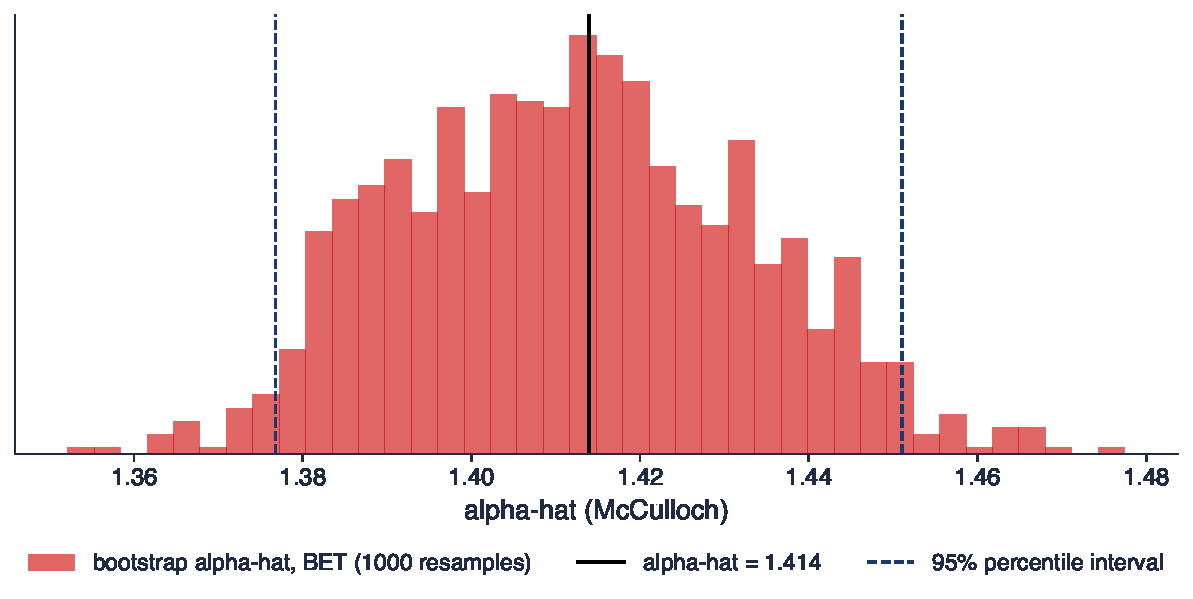
\includegraphics[width=0.96\textwidth,height=0.42\textheight,keepaspectratio]{ch3_sem_b1.pdf}
\end{center}
\vspace{-2mm}
\begin{itemize}
    \item $n = 6\,670$; quantiles $-1.93$, $-0.50$, $0.08$, $0.66$, $2.06$; $\nu_\alpha = 3.425$, $\nu_\beta = -0.006$
    \item $\hat\alpha = 1.414$, $\hat\beta = -0.011$, $\hat\gamma = 0.60\%$, $\hat\delta_0 = 0.079\%$; bootstrap SE $0.021$, 95\% interval $[1.377, 1.451]$
    \item Interpretation: $\alpha = 2$ lies far outside the interval; the BET body and tails are much wider than the Normal distribution allows
\end{itemize}\quantlet{SFM\_ch3\_seminar}{\qlurl{SFM_ch3_seminar}}
\end{frame}

\begin{frame}{B2: Three More Markets [Proposed]}
\itemsize{\footnotesize}
\begin{itemize}
\item \textbf{Question}: which of the S\&P 500, DAX and Bitcoin has the heaviest tails by McCulloch's method? Model: B1.
\item \textbf{Inputs}: S\&P 500 and DAX since 2000, Bitcoin since 2014, daily log returns in \%
\item \textbf{Tasks}
\begin{enumerate}
    \item Repeat steps 1--3 of B1 for each series.
    \item Put $\nu_\alpha$, $\hat\alpha$ with its interval, $\hat\beta$ and $\hat\gamma$ of the four series (with the BET) in one table.
    \item Interpretation: is the difference between the $\hat\alpha$ of Bitcoin and of the S\&P 500 larger than the estimation error?
\end{enumerate}
\item \textbf{Report}: one table and two sentences
\item Notebook: section B2
\end{itemize}
\end{frame}

\ifsolutions
\begin{frame}{B2: Solution [Proposed]}
\itemsize{\footnotesize}
\begin{center}
\footnotesize
\begin{tabular}{lrrrrr}
\toprule
& $\nu_\alpha$ & $\hat\alpha$ & 95\% interval & $\hat\beta$ & $\hat\gamma$ (\%) \\
\midrule
BET & $3.425$ & $1.414$ & $[1.377, 1.451]$ & $-0.011$ & $0.60$ \\
S\&P 500 & $3.338$ & $1.438$ & $[1.396, 1.475]$ & $-0.151$ & $0.54$ \\
DAX & $3.285$ & $1.455$ & $[1.416, 1.506]$ & $-0.113$ & $0.68$ \\
Bitcoin & $3.803$ & $1.322$ & $[1.275, 1.369]$ & $-0.027$ & $1.44$ \\
\bottomrule
\end{tabular}
\end{center}
\begin{itemize}
    \item Heaviest tails: Bitcoin, $\hat\alpha = 1.322$; its interval does not overlap that of the S\&P 500
    \item BET, S\&P 500 and DAX: overlapping intervals, no clear ranking
    \item $\hat\gamma$ of Bitcoin is more than twice that of the indices
\end{itemize}\quantlet{SFM\_ch3\_seminar}{\qlurl{SFM_ch3_seminar}}
\end{frame}
\fi

\begin{frame}{B3: Maximum Likelihood for the S\&P 500 [Solved]}
\itemsize{\scriptsize}
\begin{itemize}
\item \textbf{Question}: does the ML stable fit describe the S\&P 500 better than the Normal distribution, in the body and in the tails?
\item \textbf{Inputs}: S\&P 500 closes since 2000, daily log returns in \%
\item \textbf{Tasks}
\begin{enumerate}
    \item Fit the stable law by ML (S0) and report $\hat\alpha$ and $\hat\beta$ with standard errors, $\hat\gamma$, $\hat\delta_0$ and $\hat\delta_1$.
    \item Compare $\hat\alpha$ with the McCulloch estimate.
    \item Fit the Normal and the Student-t distributions and compare the AIC (Akaike information criterion, $2k - 2\ell$) of the three models.
    \item Draw the QQ plot of the data against the Normal and the stable fits.
    \item Interpretation: where does each model fail?
\end{enumerate}
\item \textbf{Report}: the estimates, three AIC values, the QQ plot and two sentences
\item Notebook: section B3
\end{itemize}
\end{frame}

\begin{frame}{B3: Solution [Solved]}
\itemsize{\scriptsize}
\begin{center}
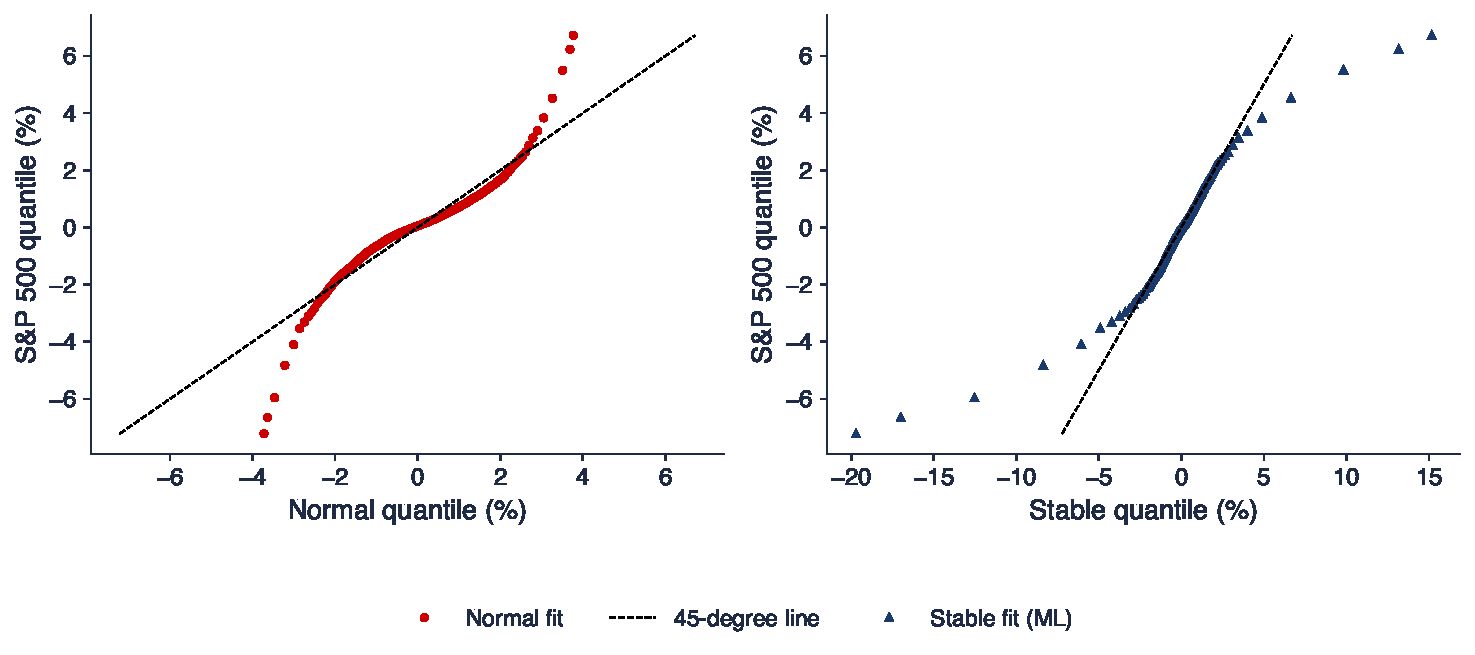
\includegraphics[width=0.96\textwidth,height=0.40\textheight,keepaspectratio]{ch3_sem_b3.pdf}
\end{center}
\vspace{-2mm}
\begin{itemize}
    \item ML: $\hat\alpha = 1.540$ (SE $0.021$, 95\% CI $[1.499, 1.581]$), $\hat\beta = -0.181$ ($0.036$), $\hat\gamma = 0.58$, $\hat\delta_0 = 0.093$, $\hat\delta_1 = 0.000$; McCulloch $\hat\alpha = 1.438$
    \item AIC: Normal 21\,650, Student-t 19\,702, stable 19\,794: the stable law beats the Normal fit by 1\,856 points, the Student-t beats the stable law by 92
    \item Interpretation: the Normal fit misses the tails (0.1\% quantile $-3.72$ vs $-7.22$ in the data); the stable fit overshoots them ($-19.70$)
\end{itemize}\quantlet{SFM\_ch3\_seminar}{\qlurl{SFM_ch3_seminar}}
\end{frame}

\begin{frame}{B4: Large Bitcoin Losses under Three Models [Proposed]}
\itemsize{\scriptsize}
\begin{itemize}
\item \textbf{Question}: which model predicts the number of large daily Bitcoin losses best? Model: B3.
\item \textbf{Inputs}: Bitcoin closes since 2014, 7 days a week, daily log returns in \%
\item \textbf{Tasks}
\begin{enumerate}
    \item Fit the Normal, Student-t and stable (ML) laws.
    \item Count the days with a loss above 10\% and above 20\%.
    \item Compute the expected number of such days under each model, $n \times P(r < -x)$.
    \item Compute VaR 1\% of the data and of each model.
    \item Interpretation: which model would you use for a margin requirement on a Bitcoin position, and why?
\end{enumerate}
\item \textbf{Report}: one table of counts, four VaR values and two sentences
\item Notebook: section B4
\end{itemize}
\end{frame}

\ifsolutions
\begin{frame}{B4: Solution [Proposed]}
\itemsize{\footnotesize}
\begin{center}
\footnotesize
\begin{tabular}{lrrrr}
\toprule
& observed & Normal & Student-t & stable \\
\midrule
loss above 10\% (days) & 56 & $8.1$ & $54.2$ & $73.9$ \\
loss above 20\% (days) & 4 & $\approx 0$ & $12.3$ & $26.9$ \\
VaR 1\% (\%) & $10.5$ & $8.0$ & $11.1$ & $14.3$ \\
\bottomrule
\end{tabular}
\end{center}
\begin{itemize}
    \item $n = 4\,384$; stable ML: $\hat\alpha = 1.410$ ($0.026$), $\hat\beta = 0.019$, $\hat\gamma = 1.54$; Student-t $\hat\nu = 2.23$
    \item Normal: far too few large losses; stable: too many beyond 20\%; Student-t: closest at 10\%, too many at 20\%
    \item Interpretation: Student-t, or the stable law as a conservative bound; never the Normal distribution
\end{itemize}\quantlet{SFM\_ch3\_seminar}{\qlurl{SFM_ch3_seminar}}
\end{frame}
\fi

\begin{frame}{B5: Does $\alpha$ Stay the Same When Returns Are Summed? [Solved]}
\itemsize{\footnotesize}
\begin{itemize}
\item \textbf{Question}: if S\&P 500 daily returns were i.i.d.\ stable, weekly and monthly returns would have the same $\alpha$; do they?
\item \textbf{Inputs}: S\&P 500 daily log returns since 2000; weekly and monthly sums
\item \textbf{Tasks}
\begin{enumerate}
    \item Compute the weekly and monthly log returns as sums of the daily ones.
    \item Compute the McCulloch $\hat\alpha$ at the three horizons.
    \item Bootstrap each $\hat\alpha$ with 500 resamples and report the 95\% intervals.
    \item Interpretation: is the pattern consistent with i.i.d.\ stable returns?
\end{enumerate}
\item \textbf{Report}: three estimates with intervals, the chart and two sentences
\item Notebook: section B5
\end{itemize}
\end{frame}

\begin{frame}{B5: Solution [Solved]}
\itemsize{\footnotesize}
\begin{center}
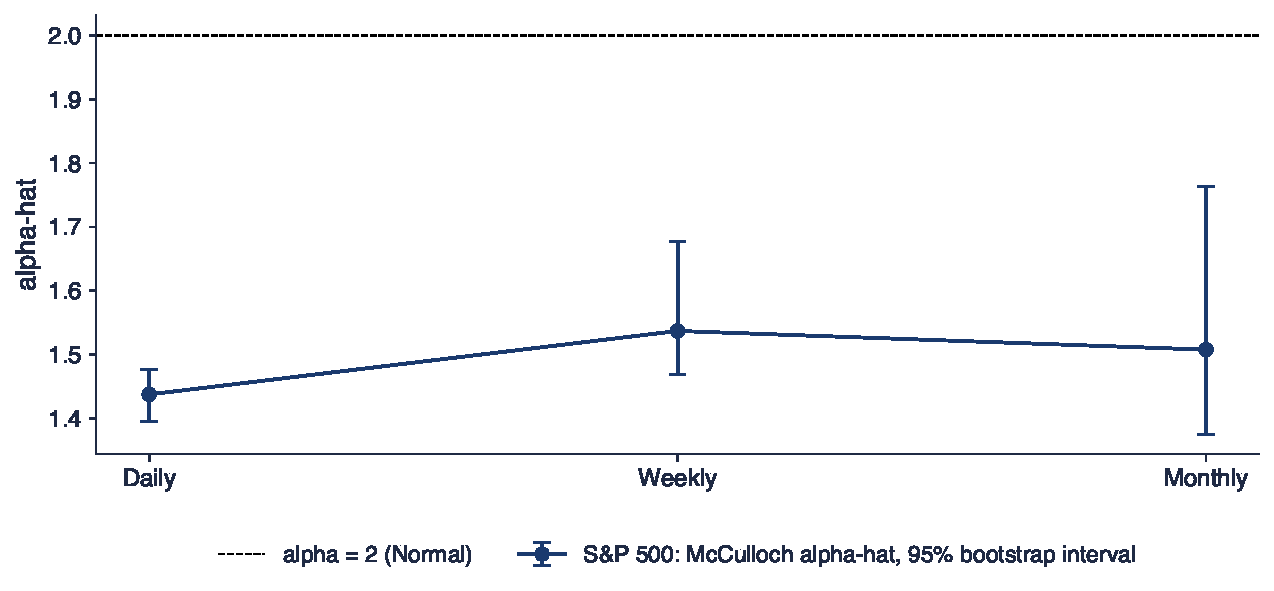
\includegraphics[width=0.96\textwidth,height=0.42\textheight,keepaspectratio]{ch3_sem_b5.pdf}
\end{center}
\vspace{-2mm}
\begin{itemize}
    \item Daily ($n = 6\,714$): $1.44$ $[1.40, 1.48]$; weekly ($1\,394$): $1.54$ $[1.47, 1.68]$; monthly ($321$): $1.51$ $[1.37, 1.76]$
    \item $\hat\alpha$ is higher for weekly than for daily returns; the monthly interval is wide and reaches up to $1.76$
    \item Interpretation: a rising $\alpha$ is a warning sign against i.i.d.\ stable returns; monthly samples are too short for a firm answer (Lecture 3 repeats the test with ML)
\end{itemize}\quantlet{SFM\_ch3\_seminar}{\qlurl{SFM_ch3_seminar}}
\end{frame}

\begin{frame}{B6: Does the Sample Variance Settle? [Proposed]}
\itemsize{\footnotesize}
\begin{itemize}
\item \textbf{Question}: is the sample variance of BET and Bitcoin returns as large and as unstable as a stable law with the fitted $\alpha$ implies? Models: B1, B5.
\item \textbf{Inputs}: BET since 2000, Bitcoin since 2014, daily log returns in \%
\item \textbf{Tasks}
\begin{enumerate}
    \item Compute the sample variance of each series over the full sample and over its first half.
    \item Simulate 200 paths of the same length from the McCulloch fit (CMS) and compute the sample variance of each path.
    \item Report the median and the 5\% and 95\% percentiles of the simulated variances, and the share below the observed one.
    \item Interpretation: what does the comparison say about the infinite-variance hypothesis?
\end{enumerate}
\item \textbf{Report}: a table with two rows and one sentence
\item Notebook: section B6
\end{itemize}
\end{frame}

\ifsolutions
\begin{frame}{B6: Solution [Proposed]}
\itemsize{\footnotesize}
\begin{center}
\footnotesize
\begin{tabular}{lrrrrrr}
\toprule
& $\hat\alpha$ & var. data & first half & sim. median & sim. 5--95\% & share below \\
\midrule
BET & $1.414$ & $2.0$ & $3.0$ & $19.2$ & $[7.3, 215.0]$ & $0\%$ \\
Bitcoin & $1.322$ & $12.1$ & $15.4$ & $213.0$ & $[63.2, 4442.0]$ & $0\%$ \\
\bottomrule
\end{tabular}
\end{center}
\begin{itemize}
    \item The observed variance is below every simulated one: real returns are far less extreme than the fitted stable law implies
    \item Interpretation: evidence against infinite variance; the variance of the first half differs from that of the full sample because volatility changes over time
\end{itemize}\quantlet{SFM\_ch3\_seminar}{\qlurl{SFM_ch3_seminar}}
\end{frame}
\fi


%=============================================================================
\section{Part C: Open Questions and AI Critique}
%=============================================================================

\begin{frame}{C1: Is $\alpha$ Constant over Time? [Proposed]}
\itemsize{\footnotesize}
\begin{itemize}
\item \textbf{Question}: do the tails of the BET and the S\&P 500 change from one five-year period to the next?
\item \textbf{Inputs}: daily log returns since 2000, split into 2000--2004, 2005--2009, 2010--2014, 2015--2019, 2020--2026; models: B1, B3
\item \textbf{Tasks}
\begin{enumerate}
    \item Compute the McCulloch $\hat\alpha$ with a bootstrap interval in each period, for each index.
    \item Say which periods differ significantly.
    \item Propose one explanation for the changes and one way to test it (for example, returns divided by a rolling volatility).
    \item Interpretation: what would a changing $\alpha$ mean for a risk model estimated on old data?
\end{enumerate}
\item \textbf{Report}: a table, a short list of significant changes and a plan for a project
\item Notebook: section C1
\end{itemize}
\end{frame}

\ifsolutions
\begin{frame}{C1: Reference Analysis [Proposed]}
\itemsize{\scriptsize}
\begin{center}
\scriptsize
\begin{tabular}{llrrr}
\toprule
Index & period & $n$ & $\hat\alpha$ & 95\% interval \\
\midrule
BET & 2000--2005 & 1238 & $1.46$ & $[1.38, 1.58]$ \\
BET & 2005--2010 & 1245 & $1.48$ & $[1.40, 1.59]$ \\
BET & 2010--2015 & 1261 & $1.52$ & $[1.42, 1.64]$ \\
BET & 2015--2020 & 1251 & $1.64$ & $[1.51, 1.81]$ \\
BET & 2020--2026 & 1675 & $1.48$ & $[1.43, 1.58]$ \\
S\&P 500 & 2000--2005 & 1254 & $1.63$ & $[1.50, 1.77]$ \\
S\&P 500 & 2005--2010 & 1258 & $1.28$ & $[1.23, 1.39]$ \\
S\&P 500 & 2010--2015 & 1258 & $1.42$ & $[1.35, 1.50]$ \\
S\&P 500 & 2015--2020 & 1257 & $1.35$ & $[1.28, 1.43]$ \\
S\&P 500 & 2020--2026 & 1687 & $1.54$ & $[1.45, 1.65]$ \\
\bottomrule
\end{tabular}
\end{center}
\begin{itemize}
    \item S\&P 500: $\hat\alpha$ between $1.28$ and $1.63$, lowest in 2005--2010 (the global financial crisis); several intervals do not overlap
    \item BET: between $1.46$ and $1.64$; the changes follow volatility regimes, a sign of volatility clustering (Chapter 9)
    \item Project directions: rolling windows, ML, returns standardised by GARCH volatility, more BVB stocks
\end{itemize}\quantlet{SFM\_ch3\_seminar}{\qlurl{SFM_ch3_seminar}}
\end{frame}
\fi

\begin{frame}{C2: Audit an AI Answer [Proposed]}
\itemsize{\scriptsize}
\begin{itemize}
    \item A student asked an AI assistant to fit a stable law to the daily S\&P 500 log returns (\%) since 2000. The answer:
    \item \aiprompt{(a) scipy's levy\_stable uses S0 by default, so loc = 0.000 is the S0 location delta0.}
    \item \aiprompt{(b) With alpha = 1.540 and gamma = 0.58, the variance of daily returns is 2 gamma\textasciicircum 2 = 0.68.}
    \item \aiprompt{(c) The scale of 20-day returns is sqrt(20) x gamma = 2.60\%.}
    \item \aiprompt{(d) Since alpha < 2, the VaR 1\% of this model does not exist.}
    \item \aiprompt{(e) Since alpha > 1, the mean daily return exists.}
    \item Tasks
    \begin{itemize}
        \item 1. For each statement, say whether it is correct; if not, give the correct statement and, where possible, the correct number from the notebook (section C2).
        \item 2. Report: a list of five verdicts with one line of justification each.
    \end{itemize}
\end{itemize}
\end{frame}

\ifsolutions
\begin{frame}{C2: Solution [Proposed]}
\itemsize{\footnotesize}
\begin{itemize}
    \item (a) Wrong: scipy uses S1 by default; $\hat\delta_1 = 0.000$ and $\hat\delta_0 = \hat\delta_1 + \hat\beta\hat\gamma\tan\frac{\pi\hat\alpha}{2} = 0.093$
    \item (b) Wrong: $2\gamma^2$ is the variance only for $\alpha = 2$; with $\alpha < 2$ the model variance is infinite; the sample variance is $1.47$
    \item (c) Wrong: under the stable model the scale grows like $20^{1/\alpha}$: $6.99 \times 0.58 = 4.07\%$, not $\sqrt{20} = 4.47$ times
    \item (d) Wrong: quantiles always exist; VaR 1\% of the fitted stable law is $4.54\%$ (it is ES that needs $\alpha > 1$, which holds here)
    \item (e) Correct: $E|X| < \infty$ because $1 < \alpha$; in S1 the mean equals $\delta_1$
\end{itemize}\quantlet{SFM\_ch3\_seminar}{\qlurl{SFM_ch3_seminar}}
\end{frame}
\fi


%=============================================================================
\section{Wrap-Up}
%=============================================================================

\begin{frame}{What You Should Take from Today}
\itemsize{\small}
\begin{itemize}
    \item A stable sum of $n$ terms scales like $n^{1/\alpha}$, faster than $\sqrt{n}$ when $\alpha < 2$
    \item Know the parameterisation: S0 and S1 differ in the location; scipy uses S1
    \item McCulloch: five quantiles and a table; ML: more precise; bootstrap for intervals
    \item Real returns: $\hat\alpha$ well below 2 at the daily horizon, yet the variance settles and $\hat\alpha$ rises with aggregation
    \item An AI answer is a draft: check the parameterisation, the scale rule and what exists for $\alpha < 2$
\end{itemize}
\end{frame}

\begin{frame}{After the Seminar}
\itemsize{\small}
\begin{itemize}
    \item Lecture 3 develops each topic of today: stability, the generalised CLT, parameters, tails, simulation, estimation and the critique
    \item Try the [Proposed] tasks in the notebook; the solutions are discussed in class
    \item C1 can grow into a team project: rolling windows, ML, more markets
    \item Reading: \refNolan, Ch.~1; \refBHW; \refMcCulloch
\end{itemize}
\end{frame}


%=============================================================================
\section{References}
%=============================================================================

\begin{frame}{References}
\itemsize{\tiny}
\begin{itemize}
    \item Borak, S., Härdle, W., Weron, R. (2005). \href{https://doi.org/10.1007/3-540-27395-6_1}{Stable distributions}. In Čížek, P., Härdle, W., Weron, R. (eds.), \textit{Statistical Tools for Finance and Insurance}, 21--44. Springer.
    \item Chambers, J.M., Mallows, C.L., Stuck, B.W. (1976). \href{https://doi.org/10.1080/01621459.1976.10480344}{A method for simulating stable random variables}. \textit{Journal of the American Statistical Association}, 71(354), 340--344.
    \item Franke, J., Härdle, W.K., Hafner, C.M. (2019). \href{https://doi.org/10.1007/978-3-030-13751-9}{\textit{Statistics of Financial Markets: An Introduction}}, 5th ed. Springer.
    \item Mandelbrot, B. (1963). \href{https://doi.org/10.1086/294632}{The variation of certain speculative prices}. \textit{Journal of Business}, 36(4), 394--419.
    \item McCulloch, J.H. (1986). \href{https://doi.org/10.1080/03610918608812563}{Simple consistent estimators of stable distribution parameters}. \textit{Communications in Statistics -- Simulation and Computation}, 15(4), 1109--1136.
    \item Nolan, J.P. (2001). \href{https://doi.org/10.1007/978-1-4612-0197-7_17}{Maximum likelihood estimation and diagnostics for stable distributions}. In Barndorff-Nielsen, O.E., Mikosch, T., Resnick, S.I. (eds.), \textit{Lévy Processes}, 379--400. Birkhäuser.
    \item Nolan, J.P. (2020). \href{https://doi.org/10.1007/978-3-030-52915-4}{\textit{Univariate Stable Distributions: Models for Heavy Tailed Data}}. Springer.
    \item Weron, R. (1996). \href{https://doi.org/10.1016/0167-7152(95)00113-1}{On the Chambers--Mallows--Stuck method for simulating skewed stable random variables}. \textit{Statistics \& Probability Letters}, 28(2), 165--171.
\end{itemize}
\end{frame}

\end{document}
